\documentclass[aspectratio=169,11pt]{beamer}

\usetheme{Madrid}
\usecolortheme{default}
\setbeamertemplate{navigation symbols}{}
\setbeamertemplate{footline}[frame number]

\usepackage{amsmath,amssymb}
\usepackage{graphicx}
\usepackage{tikz}
\usetikzlibrary{positioning,calc}
\usetikzlibrary{arrows.meta,decorations.pathmorphing}

\definecolor{RamRed}{RGB}{190,40,45}
\definecolor{RamBlue}{RGB}{30,90,180}
\definecolor{SoftGray}{RGB}{245,245,245}
\definecolor{DarkGray}{RGB}{70,70,70}
\definecolor{MapGreen}{RGB}{48,150,95}
\definecolor{MapGold}{RGB}{235,180,45}

\setbeamercolor{title}{fg=DarkGray}
\setbeamercolor{frametitle}{fg=white,bg=RamBlue}
\setbeamercolor{structure}{fg=RamBlue}

\tikzset{
  v/.style={circle,draw=black,fill=white,inner sep=1.8pt},
  edge/.style={draw=RamBlue,line width=1.25pt},
  topic/.style={draw=black!30,fill=SoftGray,rounded corners=5pt,inner sep=7pt,
    text width=5.8cm,minimum height=1.65cm,align=left},
}


\usepackage{booktabs}
\tikzset{dot/.style={circle,fill=black,inner sep=2pt}, lab/.style={circle,draw=black,fill=white,inner sep=2pt,minimum size=6mm,font=\small},selected/.style={draw=RamRed,line width=2pt}}
\title{Trees}
\subtitle{Section 1.3 of Harris--Hirst--Mossinghoff}
\author{Jeremy Quastel}
\date{}
\begin{document}
\begin{frame}[plain]{}
\large
\begin{center}{\Huge\bfseries Trees}\par\vspace{.25cm}{\Large Section 1.3}\par\vspace{.15cm}{\large Harris--Hirst--Mossinghoff, \emph{Combinatorics and Graph Theory}}\par\vspace{.35cm}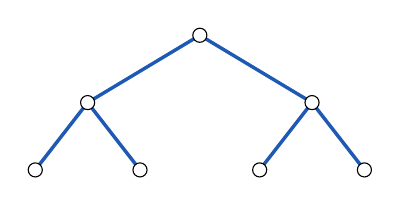
\begin{tikzpicture}[scale=0.95]
\coordinate (p1) at (0,0);
\coordinate (p2) at (-1.5,-0.9);
\coordinate (p3) at (1.5,-0.9);
\coordinate (p4) at (-2.2,-1.8);
\coordinate (p5) at (-0.8,-1.8);
\coordinate (p6) at (0.8,-1.8);
\coordinate (p7) at (2.2,-1.8);
\draw[edge] (p1) -- (p2);
\draw[edge] (p1) -- (p3);
\draw[edge] (p2) -- (p4);
\draw[edge] (p2) -- (p5);
\draw[edge] (p3) -- (p6);
\draw[edge] (p3) -- (p7);
\node[v] at (p1) {};
\node[v] at (p2) {};
\node[v] at (p3) {};
\node[v] at (p4) {};
\node[v] at (p5) {};
\node[v] at (p6) {};
\node[v] at (p7) {};
\end{tikzpicture}\par\vspace{.3cm}Jeremy Quastel\end{center}
\end{frame}

\begin{frame}[plain]{}
\large
\begin{center}{\Huge\bfseries Today's lecture}\par\vspace{.5cm}\end{center}\begin{columns}[c,onlytextwidth]\begin{column}{.48\textwidth}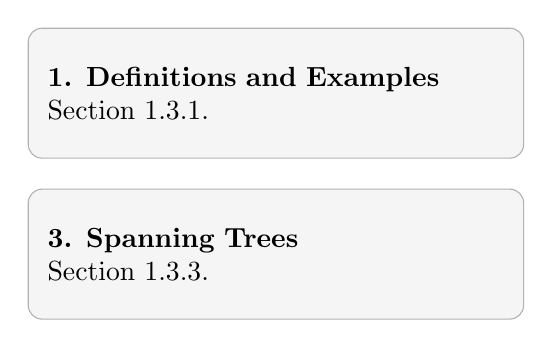
\begin{tikzpicture}\node[topic](a){\textbf{1. Definitions and Examples}\\Section 1.3.1.};\node[topic,below=.38cm of a]{\textbf{3. Spanning Trees}\\Section 1.3.3.};\end{tikzpicture}\end{column}\begin{column}{.48\textwidth}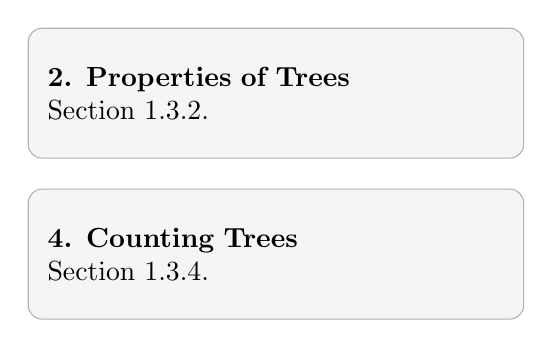
\begin{tikzpicture}\node[topic](a){\textbf{2. Properties of Trees}\\Section 1.3.2.};\node[topic,below=.38cm of a]{\textbf{4. Counting Trees}\\Section 1.3.4.};\end{tikzpicture}\end{column}\end{columns}
\end{frame}

\section{Definitions and Examples}
\begin{frame}{Definition: Trees and Forests}
\large
\begin{block}{Tree}
A \textbf{tree} is a connected graph with no cycles.
\end{block}
\begin{block}{Forest}
A \textbf{forest} is a graph whose connected components are trees. Equivalently, it is an acyclic graph.
\end{block}
\medskip
\begin{columns}[c,onlytextwidth]
\begin{column}{.32\textwidth}\centering
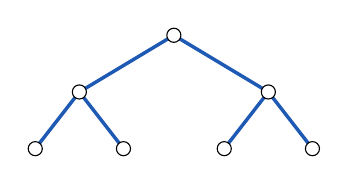
\begin{tikzpicture}[scale=0.8]
\coordinate (p1) at (0,0);
\coordinate (p2) at (-1.5,-0.9);
\coordinate (p3) at (1.5,-0.9);
\coordinate (p4) at (-2.2,-1.8);
\coordinate (p5) at (-0.8,-1.8);
\coordinate (p6) at (0.8,-1.8);
\coordinate (p7) at (2.2,-1.8);
\draw[edge] (p1) -- (p2);
\draw[edge] (p1) -- (p3);
\draw[edge] (p2) -- (p4);
\draw[edge] (p2) -- (p5);
\draw[edge] (p3) -- (p6);
\draw[edge] (p3) -- (p7);
\node[v] at (p1) {};
\node[v] at (p2) {};
\node[v] at (p3) {};
\node[v] at (p4) {};
\node[v] at (p5) {};
\node[v] at (p6) {};
\node[v] at (p7) {};
\end{tikzpicture}
\par\medskip{\normalsize A: A tree}
\end{column}
\begin{column}{.32\textwidth}\centering
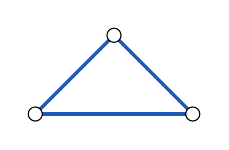
\begin{tikzpicture}[scale=1]
\coordinate (p1) at (0,0);
\coordinate (p2) at (1,1);
\coordinate (p3) at (2,0);
\draw[edge] (p1) -- (p2);
\draw[edge] (p2) -- (p3);
\draw[edge] (p3) -- (p1);
\node[v] at (p1) {};
\node[v] at (p2) {};
\node[v] at (p3) {};
\end{tikzpicture}
\par\medskip{\normalsize B: Contains a cycle}
\end{column}
\begin{column}{.32\textwidth}\centering
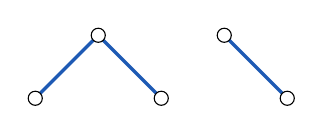
\begin{tikzpicture}[scale=0.8]
\coordinate (p1) at (0,0);
\coordinate (p2) at (1,1);
\coordinate (p3) at (2,0);
\coordinate (p4) at (3,1);
\coordinate (p5) at (4,0);
\draw[edge] (p1) -- (p2);
\draw[edge] (p2) -- (p3);
\draw[edge] (p4) -- (p5);
\node[v] at (p1) {};
\node[v] at (p2) {};
\node[v] at (p3) {};
\node[v] at (p4) {};
\node[v] at (p5) {};
\end{tikzpicture}
\par\medskip{\normalsize C: A forest with two components}
\end{column}
\end{columns}
\end{frame}

\begin{frame}{Definition: Leaves}
\large
\begin{block}{Leaf}
A vertex of degree $1$ in a tree is called a \textbf{leaf}.
\end{block}
\begin{center}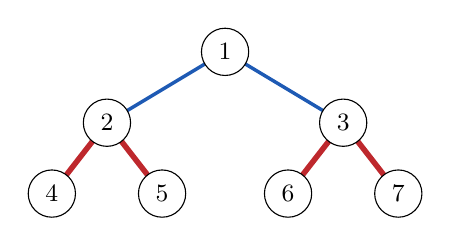
\begin{tikzpicture}[scale=1]
\coordinate (p1) at (0,0);
\coordinate (p2) at (-1.5,-0.9);
\coordinate (p3) at (1.5,-0.9);
\coordinate (p4) at (-2.2,-1.8);
\coordinate (p5) at (-0.8,-1.8);
\coordinate (p6) at (0.8,-1.8);
\coordinate (p7) at (2.2,-1.8);
\draw[edge] (p1) -- (p2);
\draw[edge] (p1) -- (p3);
\draw[selected] (p2) -- (p4);
\draw[selected] (p2) -- (p5);
\draw[selected] (p3) -- (p6);
\draw[selected] (p3) -- (p7);
\node[lab] at (p1) {1};
\node[lab] at (p2) {2};
\node[lab] at (p3) {3};
\node[lab] at (p4) {4};
\node[lab] at (p5) {5};
\node[lab] at (p6) {6};
\node[lab] at (p7) {7};
\end{tikzpicture}\end{center}\begin{center}The leaves are $4,5,6,7$.\end{center}$K_1$ is a tree, but its only vertex has degree $0$ and is not a leaf.
\end{frame}

\begin{frame}{Types of Trees of Order 6 or less}
\centering
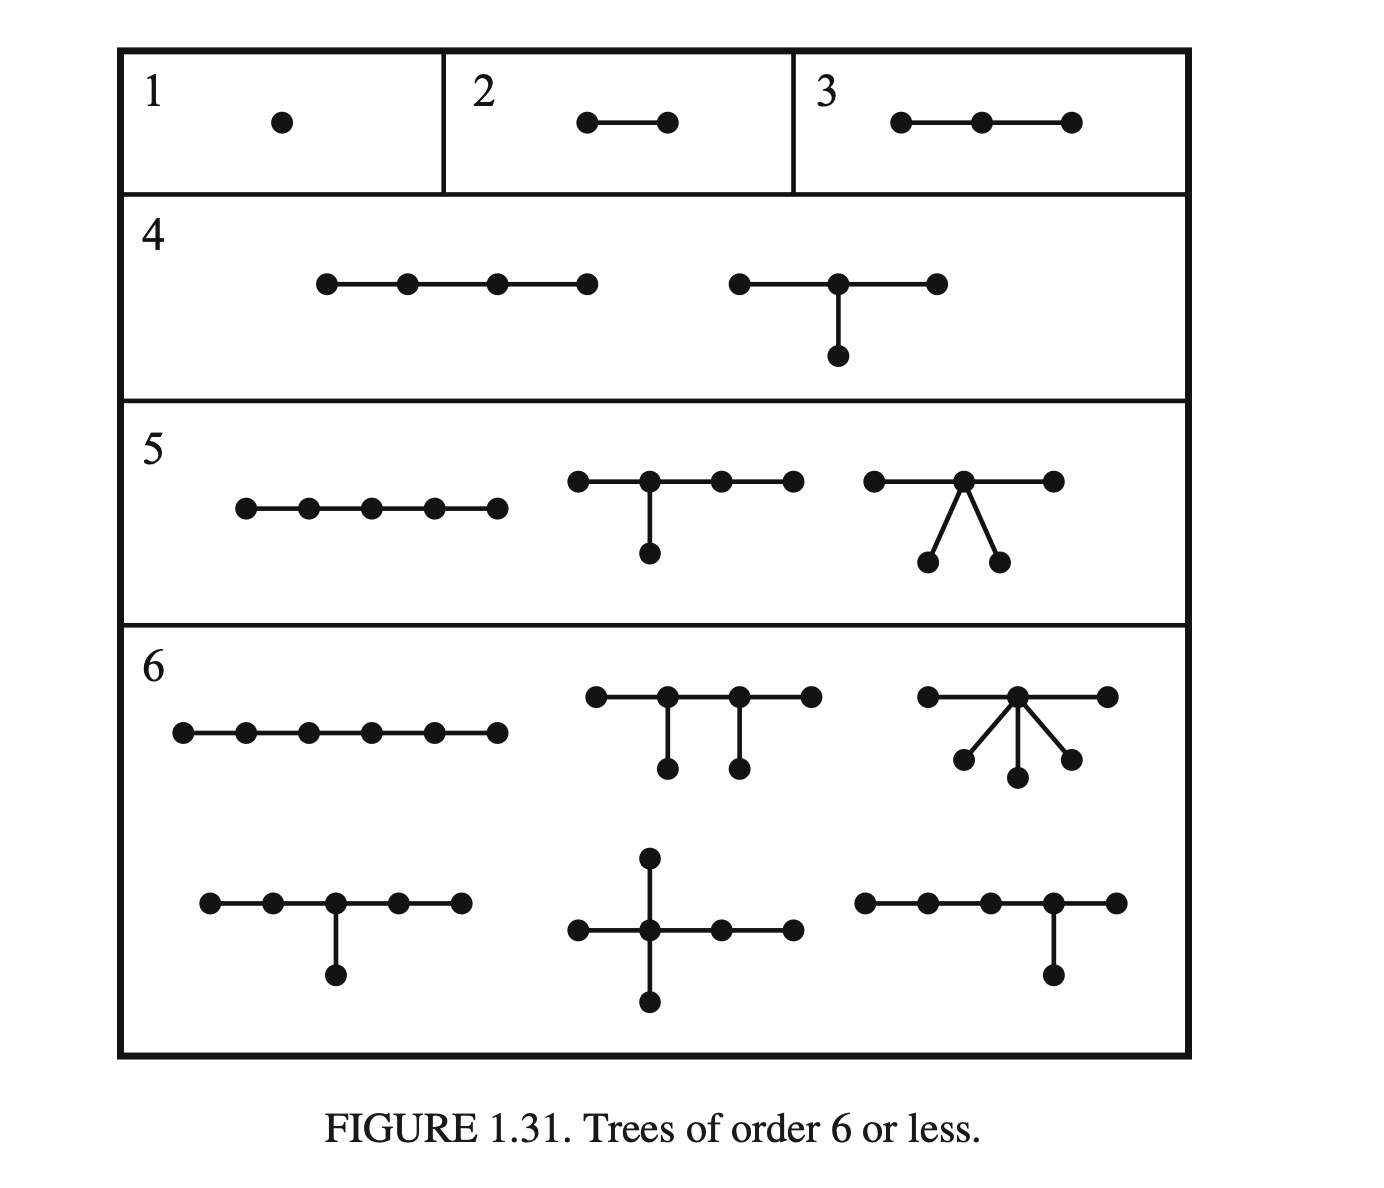
\includegraphics[height=6.1cm,keepaspectratio]{figure_1_31.png}
\par\vfill
{\tiny\raggedright Source: Harris, Hirst, and Mossinghoff, \emph{Combinatorics and Graph Theory}, 2nd ed., Springer, 2008, p.~32, Figure~1.31.\par}
\end{frame}

\begin{frame}[t]{Application 1: Possible Outcomes}
\large
A branching diagram records the possible results of successive steps in an experiment, such as tossing a coin and rolling a die.
\par\medskip\centering
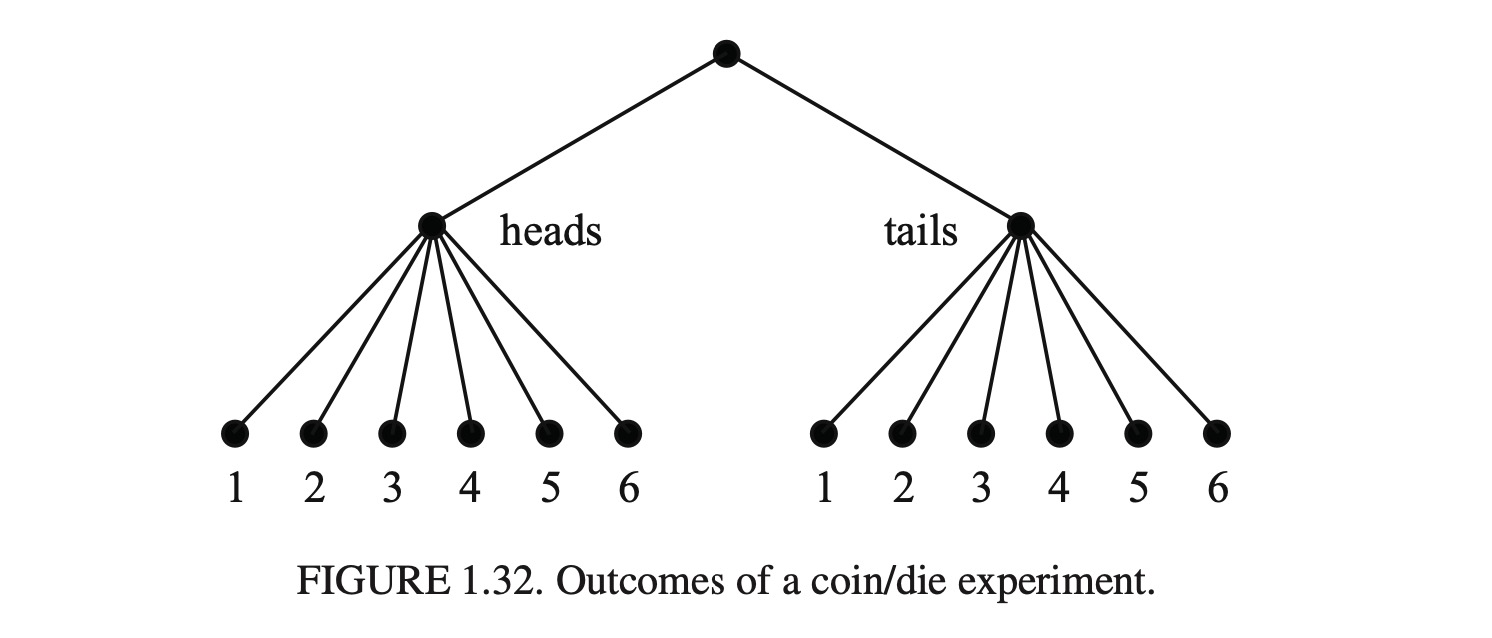
\includegraphics[width=0.94\textwidth,height=4.75cm,keepaspectratio]{figure_1_32.png}
\par\vfill
{\tiny\raggedright Source: Harris, Hirst, and Mossinghoff, \emph{Combinatorics and Graph Theory}, 2nd ed., Springer, 2008, p.~32, Figure~1.32.\par}
\end{frame}

\begin{frame}[t]{Application 2: Computer Algorithms}
\large
Trees organize searches and sorting procedures, and represent the sequence of decisions made by an algorithm.
\par\medskip\centering
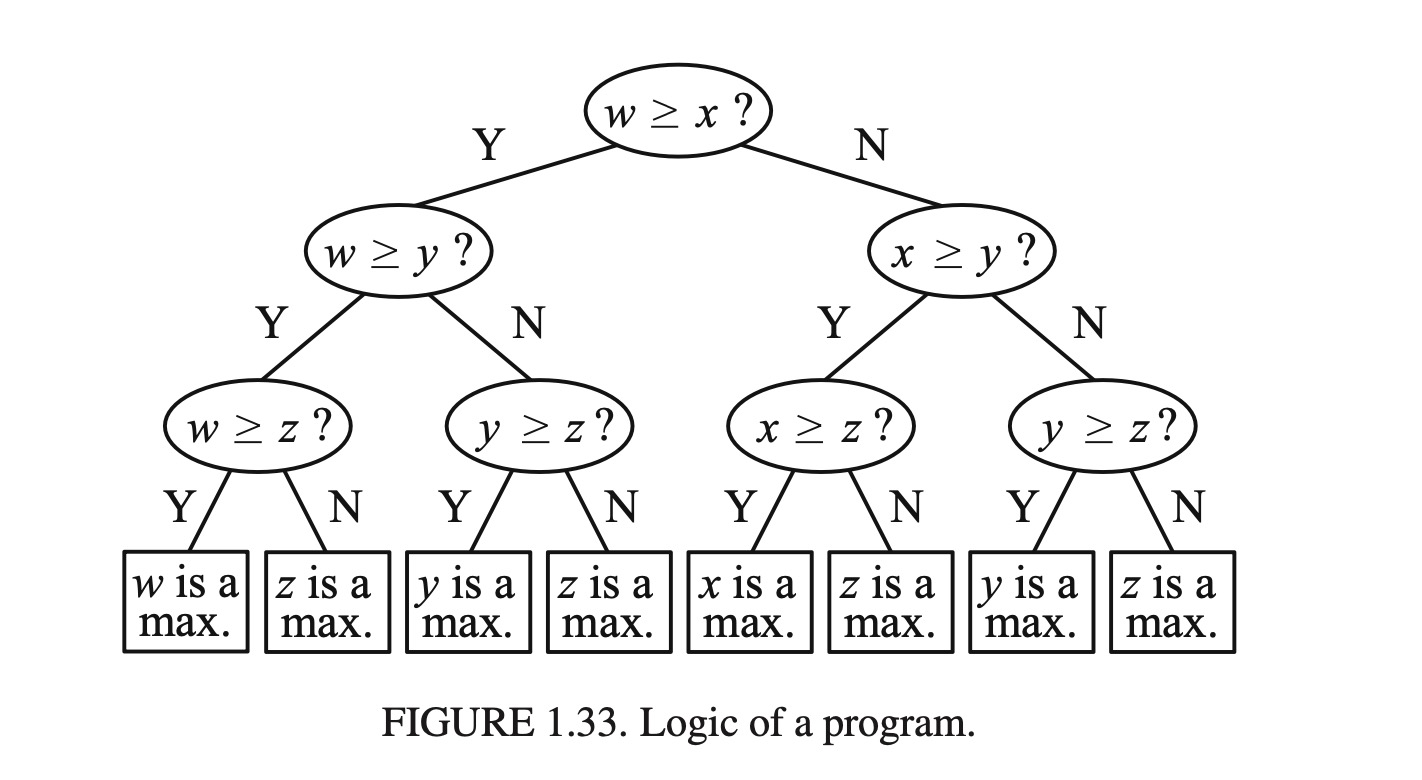
\includegraphics[width=0.94\textwidth,height=4.75cm,keepaspectratio]{figure_1_33.png}
\par\vfill
{\tiny\raggedright Source: Harris, Hirst, and Mossinghoff, \emph{Combinatorics and Graph Theory}, 2nd ed., Springer, 2008, p.~33, Figure~1.33.\par}
\end{frame}

\begin{frame}[t]{Application 3: Chemical Compounds}
\large
Trees can model the atoms and bonds in acyclic saturated hydrocarbons. Carbon atoms have degree $4$, and hydrogen atoms are leaves.
\par\medskip\centering
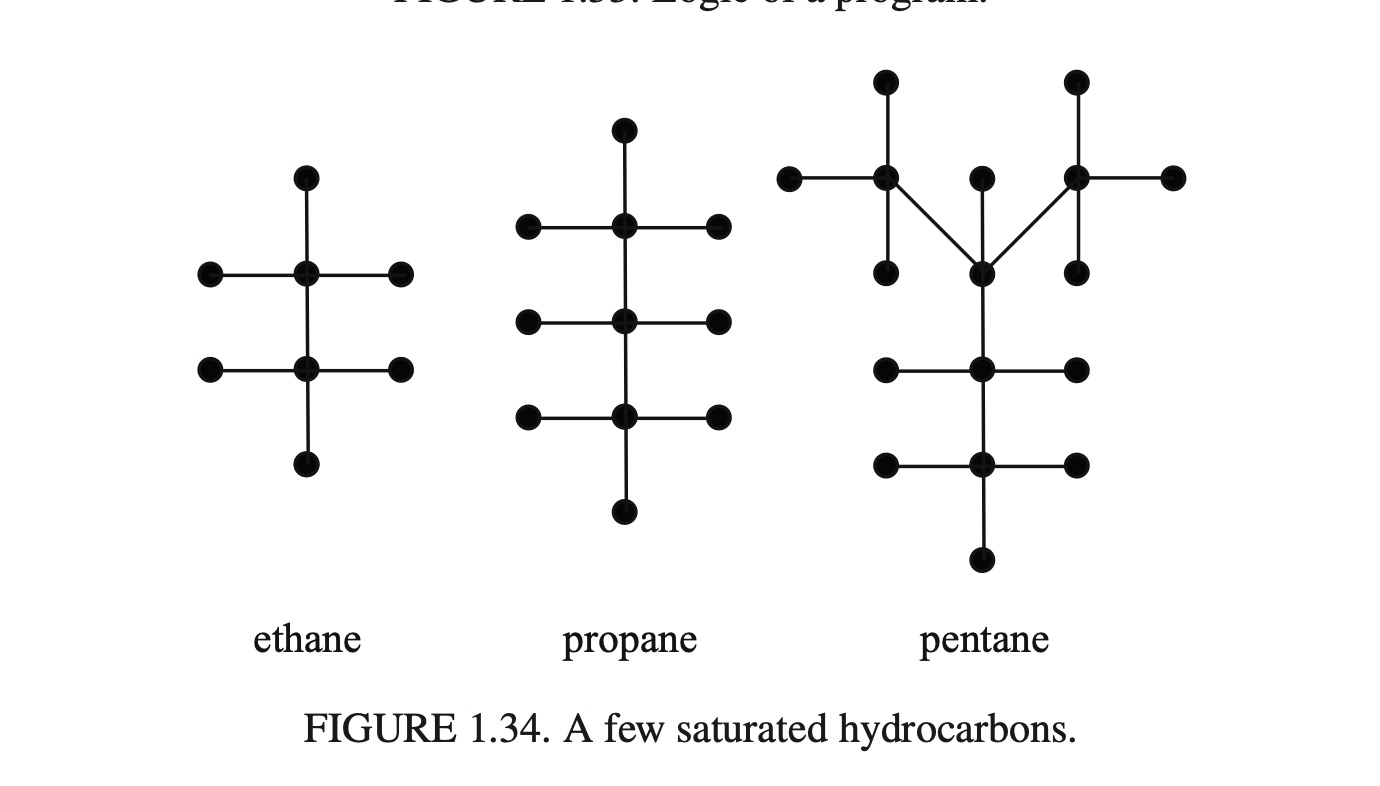
\includegraphics[width=0.94\textwidth,height=4.75cm,keepaspectratio,trim=0 0 0 16,clip]{figure_1_34.png}
\par\vfill
{\tiny\raggedright Source: Harris, Hirst, and Mossinghoff, \emph{Combinatorics and Graph Theory}, 2nd ed., Springer, 2008, p.~33, Figure~1.34.\par}
\end{frame}

\begin{frame}[t]{Application 4: Tournament Brackets}
\large
A tree records how winners advance through successive rounds of a single-elimination tournament.
\par\medskip\centering
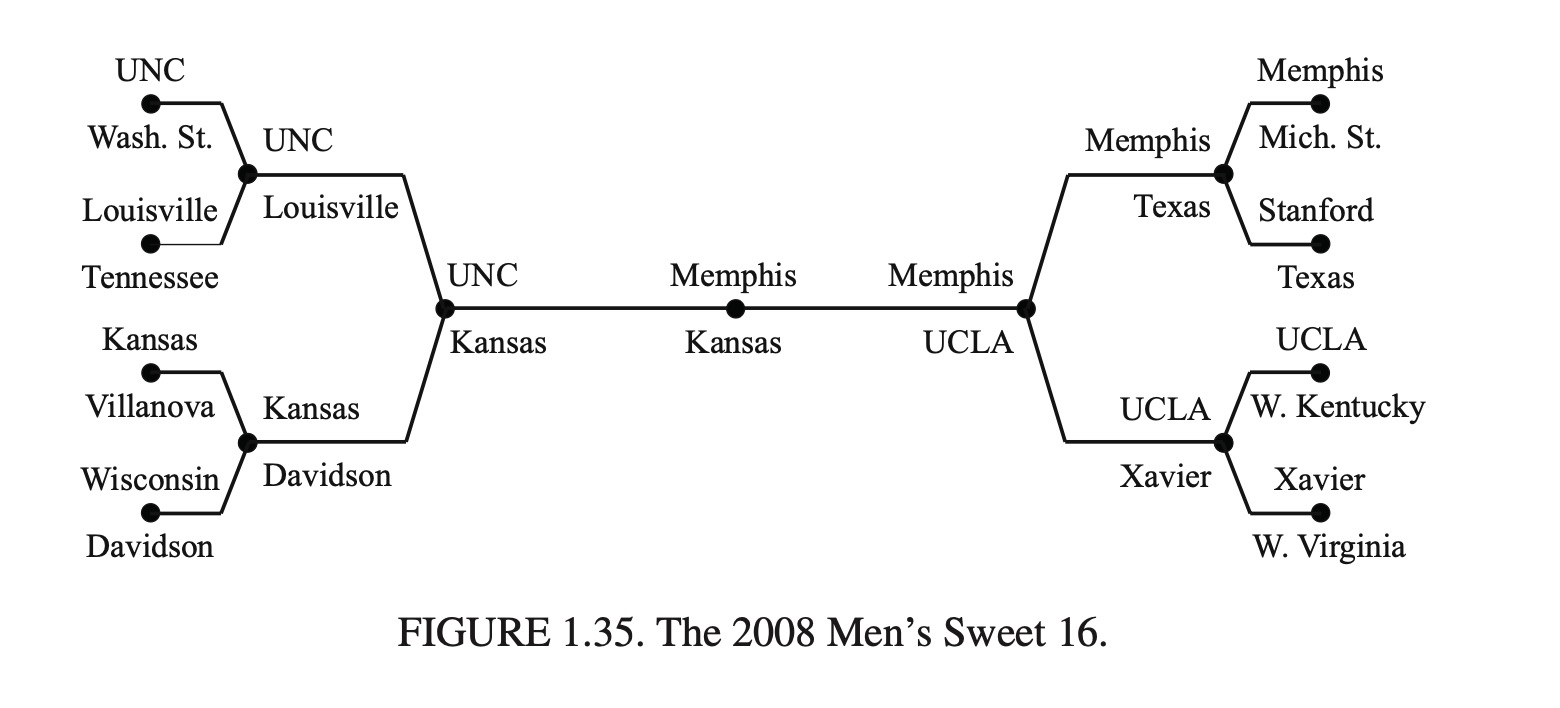
\includegraphics[width=0.94\textwidth,height=4.75cm,keepaspectratio]{figure_1_35.png}
\par\vfill
{\tiny\raggedright Source: Harris, Hirst, and Mossinghoff, \emph{Combinatorics and Graph Theory}, 2nd ed., Springer, 2008, p.~33, Figure~1.35.\par}
\end{frame}











\section{Properties of Trees}
\begin{frame}{Properties of Trees}
\large
\begin{block}{Question}
Draw a tree with $10$ vertices. How many edges does it have?
\end{block}
\par\bigskip Does the answer depend on the shape of your tree?
\end{frame}

\begin{frame}{A Useful Observation: Unique Paths}
\large
\begin{block}{Unique paths}
In a tree, each pair of distinct vertices is joined by exactly one path.
\end{block}
\begin{enumerate}
\setlength{\itemsep}{0.22cm}
\item Connectedness gives at least one path.
\item If there were two different paths, take a point where they separate and their first subsequent meeting. The two segments form a cycle.
\end{enumerate}\par\medskip\textbf{Consequence.} Every edge of a tree is a bridge. Deleting it leaves exactly two components.
\end{frame}

\begin{frame}{Theorem: Counting Edges}
\large
\begin{block}{Theorem 1.10}
A tree with $n$ vertices has exactly $n-1$ edges.
\end{block}
\begin{center}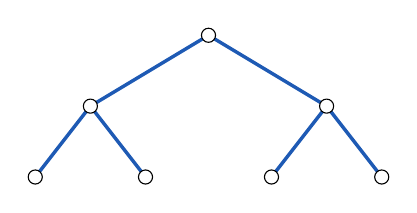
\begin{tikzpicture}[scale=1]
\coordinate (p1) at (0,0);
\coordinate (p2) at (-1.5,-0.9);
\coordinate (p3) at (1.5,-0.9);
\coordinate (p4) at (-2.2,-1.8);
\coordinate (p5) at (-0.8,-1.8);
\coordinate (p6) at (0.8,-1.8);
\coordinate (p7) at (2.2,-1.8);
\draw[edge] (p1) -- (p2);
\draw[edge] (p1) -- (p3);
\draw[edge] (p2) -- (p4);
\draw[edge] (p2) -- (p5);
\draw[edge] (p3) -- (p6);
\draw[edge] (p3) -- (p7);
\node[v] at (p1) {};
\node[v] at (p2) {};
\node[v] at (p3) {};
\node[v] at (p4) {};
\node[v] at (p5) {};
\node[v] at (p6) {};
\node[v] at (p7) {};
\end{tikzpicture}\end{center}\begin{center}$7$ vertices, $6$ edges.\end{center}
\end{frame}

\begin{frame}{Proof of Theorem 1.10}
\begin{block}{Theorem 1.10}
\large A tree with $n$ vertices has exactly $n-1$ edges.
\end{block}
\begin{block}{Proof}
\normalsize
Induct on $n$. For $n=1$, the tree is $K_1$ and has $0$ edges. Assume the result for all smaller trees, and let $T$ have $n\ge2$ vertices.
\par\smallskip
Delete any edge $e$. Since $T$ has no cycles, $T-e$ consists of two trees $T_1,T_2$, with orders $n_1,n_2<n$ and $n_1+n_2=n$. By induction, they have $n_1-1$ and $n_2-1$ edges. Restoring $e$ gives
\[
|E(T)|=(n_1-1)+(n_2-1)+1=n-1.\qquad\square
\]
\end{block}
\vspace{-0.1cm}
\centering
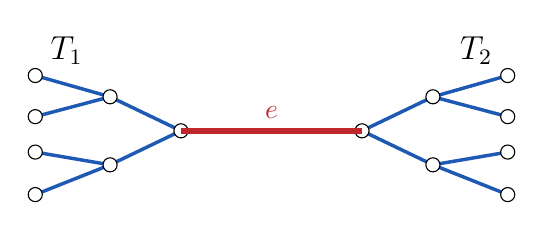
\begin{tikzpicture}[x=1cm,y=0.9cm]
\coordinate (a0) at (-1.15,0);
\coordinate (a1) at (-2.05,0.48);
\coordinate (a2) at (-2.05,-0.48);
\coordinate (a3) at (-3.0,0.78);
\coordinate (a4) at (-3.0,0.2);
\coordinate (a5) at (-3.0,-0.3);
\coordinate (a6) at (-3.0,-0.9);
\draw[edge] (a0)--(a1);
\draw[edge] (a0)--(a2);
\draw[edge] (a1)--(a3);
\draw[edge] (a1)--(a4);
\draw[edge] (a2)--(a5);
\draw[edge] (a2)--(a6);
\node[v] at (a0) {};
\node[v] at (a1) {};
\node[v] at (a2) {};
\node[v] at (a3) {};
\node[v] at (a4) {};
\node[v] at (a5) {};
\node[v] at (a6) {};
\coordinate (b0) at (1.15,0);
\coordinate (b1) at (2.05,0.48);
\coordinate (b2) at (2.05,-0.48);
\coordinate (b3) at (3.0,0.78);
\coordinate (b4) at (3.0,0.2);
\coordinate (b5) at (3.0,-0.3);
\coordinate (b6) at (3.0,-0.9);
\draw[edge] (b0)--(b1);
\draw[edge] (b0)--(b2);
\draw[edge] (b1)--(b3);
\draw[edge] (b1)--(b4);
\draw[edge] (b2)--(b5);
\draw[edge] (b2)--(b6);
\node[v] at (b0) {};
\node[v] at (b1) {};
\node[v] at (b2) {};
\node[v] at (b3) {};
\node[v] at (b4) {};
\node[v] at (b5) {};
\node[v] at (b6) {};
\draw[selected] (a0)--node[above,text=RamRed]{$e$}(b0);
\node[font=\large] at (-2.6,1.13) {$T_1$};
\node[font=\large] at (2.6,1.13) {$T_2$};
\end{tikzpicture}
\par\vfill

\end{frame}

\begin{frame}{Theorem: Counting Edges in a Forest}
\large
\begin{block}{Theorem 1.11}
A forest with $n$ vertices and $k$ components has $n-k$ edges.
\end{block}
\textbf{Proof.} If the components have orders $n_1,\ldots,n_k$, then\[|E(F)|=\sum_{i=1}^k(n_i-1)=n-k.\qquad\square\]\begin{block}{Example}
A forest with $12$ vertices and $9$ edges has $3$ components.
\end{block}

\end{frame}

\begin{frame}[t]{Theorem: Connectedness and Edge Count}
\large
\begin{block}{Theorem 1.12}
A graph on $n$ vertices is a tree if and only if it is connected and has $n-1$ edges.
\end{block}
\end{frame}

\begin{frame}[t]{Theorem: Connectedness and Edge Count}
\large
\begin{block}{Theorem 1.12}
A graph on $n$ vertices is a tree if and only if it is connected and has $n-1$ edges.
\end{block}
\begin{block}{Proof}
\normalsize
\textbf{Forward direction.} A tree is connected by definition and has $n-1$ edges by Theorem~1.10.
\par\medskip
\textbf{Reverse direction.} Suppose $G$ is connected and has $n-1$ edges. If $G$ contains a cycle, delete one edge from that cycle. This preserves connectedness.
\par\medskip
Continue deleting cycle edges until no cycle remains. The resulting graph is a tree on the same $n$ vertices. If any edge was deleted, this tree has fewer than $n-1$ edges, contradicting Theorem~1.10.
\par\medskip
Thus $G$ is acyclic and connected, so it is a tree.\hfill$\square$
\end{block}
\end{frame}

\begin{frame}[t]{Theorem: Acyclicity and Edge Count}
\large
\begin{block}{Theorem 1.13}
A graph on $n$ vertices is a tree if and only if it is acyclic and has $n-1$ edges.
\end{block}
\end{frame}

\begin{frame}[t]{Theorem: Acyclicity and Edge Count}
\large
\begin{block}{Theorem 1.13}
A graph on $n$ vertices is a tree if and only if it is acyclic and has $n-1$ edges.
\end{block}
\begin{block}{Proof}
\normalsize
\textbf{Forward direction.} A tree is acyclic by definition and has $n-1$ edges by Theorem~1.10.
\par\medskip
\textbf{Reverse direction.} Suppose $G$ is acyclic and has $n-1$ edges. Since $G$ is acyclic, it is a forest. Let $k$ be its number of components.
\par\medskip
By Theorem~1.11, a forest with $n$ vertices and $k$ components has $n-k$ edges. Hence
\[
n-1=|E(G)|=n-k,
\]
so $k=1$. Thus $G$ is connected and acyclic, and therefore is a tree.\hfill$\square$
\end{block}
\end{frame}

\begin{frame}[t]{Theorem: Trees Have Leaves}
\large
\begin{block}{Theorem 1.14}
Every tree with at least two vertices has at least two leaves.
\end{block}
\end{frame}

\begin{frame}[t]{Theorem: Trees Have Leaves}
\large
\begin{block}{Theorem 1.14}
Every tree with at least two vertices has at least two leaves.
\end{block}
\begin{block}{Proof}
\small
Induct on the number $n$ of vertices. For $n=2$, both vertices are leaves. Suppose $n\ge3$ and the result holds for smaller trees.
\par\smallskip
\textbf{Case 1: Every edge meets a leaf.} Choose two distinct edges. Their leaf endpoints are distinct, giving two leaves.
\par\smallskip
\textbf{Case 2: Some edge $uv$ has no leaf endpoint.} Delete $uv$. The resulting trees $T_1,T_2$ each have at least two vertices and fewer than $n$. By induction, each has at least two leaves. Choose a leaf of $T_1$ other than $u$ and a leaf of $T_2$ other than $v$. Both remain leaves when $uv$ is restored.\hfill$\square$
\end{block}
\vspace{-0.08cm}
{\centering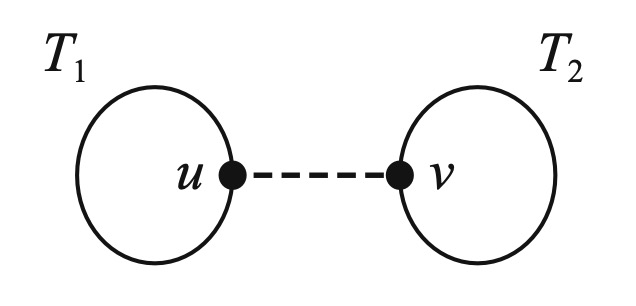
\includegraphics[height=1.45cm]{figure_leaves_proof.png}\par}
\vfill
{\tiny\raggedright Figure source: Harris, Hirst, and Mossinghoff, \emph{Combinatorics and Graph Theory}, 2nd ed., Springer, 2008, \S1.3.2, proof of Theorem~1.14.\par}
\end{frame}



\begin{frame}{Another Proof: A Longest Path}
\large
Choose a longest path $v_0,v_1,\ldots,v_r$ in the tree.\begin{center}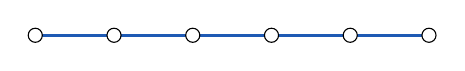
\begin{tikzpicture}[scale=1]
\coordinate (p0) at (0,0);
\coordinate (p1) at (1,0);
\coordinate (p2) at (2,0);
\coordinate (p3) at (3,0);
\coordinate (p4) at (4,0);
\coordinate (p5) at (5,0);
\draw[edge] (p0) -- (p1);
\draw[edge] (p1) -- (p2);
\draw[edge] (p2) -- (p3);
\draw[edge] (p3) -- (p4);
\draw[edge] (p4) -- (p5);
\node[v] at (p0) {};
\node[v] at (p1) {};
\node[v] at (p2) {};
\node[v] at (p3) {};
\node[v] at (p4) {};
\node[v] at (p5) {};
\end{tikzpicture}\end{center}\begin{enumerate}
\setlength{\itemsep}{0.22cm}
\item If $v_0$ had a neighbor outside the path, we could extend it.
\item If $v_0$ had a neighbor on the path other than $v_1$, there would be a cycle.
\end{enumerate}\par\medskip So $v_0$ is a leaf. The same argument applies to $v_r$.\hfill$\square$
\end{frame}





\begin{frame}[t]{Theorem: The Center of a Tree}
\large
\begin{block}{Theorem 1.15}
The center of a tree consists of one vertex or two adjacent vertices.
\end{block}
\begin{block}{Proof idea}
\normalsize
Removing all leaves of a tree with at least three vertices does not change its center. Repeat until only one vertex or two adjacent vertices remain.
\end{block}
\vspace{0.3cm}
{\centering
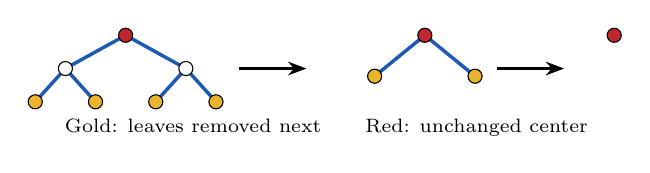
\begin{tikzpicture}[x=0.85cm,y=0.65cm]
\foreach \x/\y/\n in {0/0/a,-.9/-.65/b,.9/-.65/c,-1.35/-1.3/d,-.45/-1.3/e,.45/-1.3/f,1.35/-1.3/g}
  \coordinate (\n) at (\x,\y);
\foreach \u/\w in {a/b,a/c,b/d,b/e,c/f,c/g} \draw[edge] (\u)--(\w);
\foreach \n in {b,c} \node[v] at (\n) {};
\foreach \n in {d,e,f,g} \node[v,fill=MapGold] at (\n) {};
\node[v,fill=RamRed] at (a) {};
\draw[-{Stealth},thick] (1.7,-.65)--(2.7,-.65);
\begin{scope}[xshift=3.8cm]
\draw[edge] (-.75,-.8)--(0,0)--(.75,-.8);
\node[v,fill=RamRed] at (0,0) {};
\node[v,fill=MapGold] at (-.75,-.8) {};
\node[v,fill=MapGold] at (.75,-.8) {};
\end{scope}
\draw[-{Stealth},thick] (5.55,-.65)--(6.55,-.65);
\node[v,fill=RamRed] at (7.3,0) {};
\node[font=\scriptsize] at (3,-1.8) {Gold: leaves removed next\qquad Red: unchanged center};
\end{tikzpicture}\par}
\end{frame}

\begin{frame}[t]{Theorem: The Center of a Tree}
\large
\begin{block}{Theorem 1.15}
The center of a tree consists of one vertex or two adjacent vertices.
\end{block}
\begin{block}{Proof}
\small
The result is immediate for $K_1$ and $K_2$. Let $T$ have at least three vertices, and remove all its leaves to obtain a nonempty tree $T'$.
\par\smallskip
No leaf is central: its neighbor has smaller eccentricity. For each remaining vertex $v$, every longest path starting at $v$ ends at a leaf; pruning shortens its maximum length by exactly one. Hence $\operatorname{ecc}_{T'}(v)=\operatorname{ecc}_T(v)-1$.
All remaining eccentricities decrease equally, so $T$ and $T'$ have the same center. Repeat while there are at least three vertices. The process ends at $K_1$ or $K_2$, whose one or two adjacent vertices form the original center.\hfill$\square$
\par\smallskip
{\centering
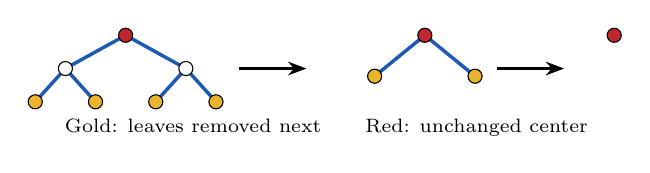
\begin{tikzpicture}[x=0.85cm,y=0.65cm]
\foreach \x/\y/\n in {0/0/a,-.9/-.65/b,.9/-.65/c,-1.35/-1.3/d,-.45/-1.3/e,.45/-1.3/f,1.35/-1.3/g}
  \coordinate (\n) at (\x,\y);
\foreach \u/\w in {a/b,a/c,b/d,b/e,c/f,c/g} \draw[edge] (\u)--(\w);
\foreach \n in {b,c} \node[v] at (\n) {};
\foreach \n in {d,e,f,g} \node[v,fill=MapGold] at (\n) {};
\node[v,fill=RamRed] at (a) {};
\draw[-{Stealth},thick] (1.7,-.65)--(2.7,-.65);
\begin{scope}[xshift=3.8cm]
\draw[edge] (-.75,-.8)--(0,0)--(.75,-.8);
\node[v,fill=RamRed] at (0,0) {};
\node[v,fill=MapGold] at (-.75,-.8) {};
\node[v,fill=MapGold] at (.75,-.8) {};
\end{scope}
\draw[-{Stealth},thick] (5.55,-.65)--(6.55,-.65);
\node[v,fill=RamRed] at (7.3,0) {};
\node[font=\scriptsize] at (3,-1.8) {Gold: leaves removed next\qquad Red: unchanged center};
\end{tikzpicture}\par}
\end{block}
\end{frame}

\begin{frame}{Theorem: Finding Trees Inside Other Graphs}
\large
\begin{block}{Theorem 1.16}
Let $T$ be a tree with $k$ edges. Every nonempty graph $G$ with $\delta(G)\ge k$ contains a subgraph isomorphic to $T$.
\end{block}
\par\medskip Equivalently, $G$ contains every tree on at most $\delta(G)+1$ vertices.\begin{block}{Remark}
The copy need not be an induced subgraph. We may leave out extra edges of $G$.
\end{block}

\end{frame}

\begin{frame}[t]{Theorem: Finding Trees Inside Other Graphs}
\large
\begin{block}{Theorem 1.16}
Let $T$ be a tree with $k$ edges. Every nonempty graph $G$ with $\delta(G)\ge k$ contains a subgraph isomorphic to $T$.
\end{block}
\end{frame}

\begin{frame}[t]{Theorem: Finding Trees Inside Other Graphs}
\large
\begin{block}{Theorem 1.16}
Let $T$ be a tree with $k$ edges. Every nonempty graph $G$ with $\delta(G)\ge k$ contains a subgraph isomorphic to $T$.
\end{block}
\begin{block}{Proof}
\small
Induct on $k$. For $k=0$, any vertex of $G$ gives a copy of $T$. Suppose $k\ge1$ and the result holds for trees with $k-1$ edges.
\par\smallskip
Choose a leaf $v$ of $T$ with neighbor $w$. By induction, $G$ contains a copy of $T-v$, which has $k$ vertices. Identify $w$ with its image in this copy.
\par\smallskip
Since $\deg_G(w)\ge k$ and only $k-1$ other vertices lie in the copy, $w$ has a neighbor $u$ outside it. Adding $u$ and the edge $uw$ gives a subgraph isomorphic to $T$, with $u$ representing $v$.\hfill$\square$
\par\smallskip
{\centering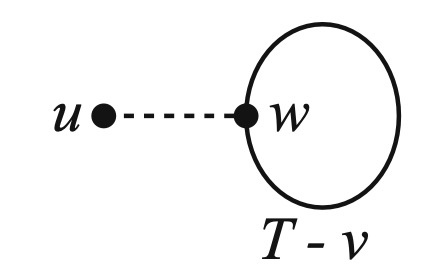
\includegraphics[height=1.5cm]{figure_tree_embedding_proof.png}\par}
\end{block}
\vfill
{\tiny\raggedright Figure source: Harris, Hirst, and Mossinghoff, \emph{Combinatorics and Graph Theory}, 2nd ed., Springer, 2008, \S1.3.2, proof of Theorem~1.16.\par}
\end{frame}

\begin{frame}{Definition: Spanning Tree}
\large
\begin{block}{Spanning tree}
A \textbf{spanning tree} of $G$ is a subgraph $T$ that is a tree and satisfies $V(T)=V(G)$.
\end{block}
\par\medskip Every connected graph has a spanning tree: delete cycle edges until no cycle remains.\par\bigskip A spanning tree on $n$ vertices always has $n-1$ edges.\par\bigskip A disconnected graph has no spanning tree.
\end{frame}

\begin{frame}[t]{Example: Planning Railroad Track}
\begin{columns}[T,onlytextwidth]
\begin{column}{0.44\textwidth}
\normalsize
A railroad network must connect all eight cities shown. The edges represent possible track links, with a weight assigned to each link.
\par\medskip
We want every city to be reachable from every other city while minimizing the total weight of the selected links.
\par\medskip
A cycle would be unnecessary: removing one of its edges preserves connectivity and reduces the total weight.
\end{column}
\begin{column}{0.54\textwidth}
\centering
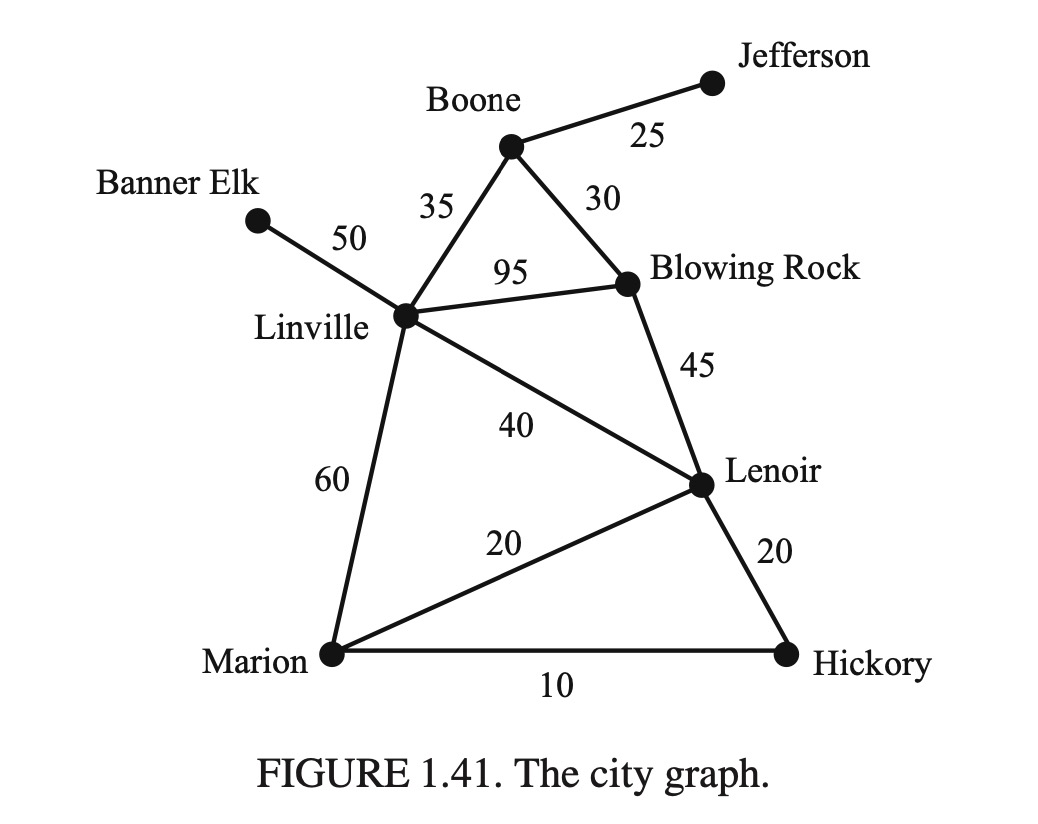
\includegraphics[width=\linewidth,height=4.7cm,keepaspectratio]{figure_1_41.png}
\end{column}
\end{columns}
\begin{block}{Goal}
\normalsize Find a \textbf{minimum weight spanning tree} of the city graph.
\end{block}
\vfill
{\tiny\raggedright Figure source: Harris, Hirst, and Mossinghoff, \emph{Combinatorics and Graph Theory}, 2nd ed., Springer, 2008, Figure~1.41.\par}
\end{frame}

\begin{frame}{Definition: Minimum Weight Spanning Tree}
\large
\begin{block}{Weighted graph}
A weight function assigns a number $w(e)\ge0$ to each edge $e$.
\end{block}
\begin{block}{Minimum weight spanning tree}
A spanning tree $T$ is a \textbf{minimum weight spanning tree} if it minimizes\[w(T)=\sum_{e\in E(T)}w(e)\]among all spanning trees of $G$.
\end{block}
\par\medskip Different spanning trees can achieve the same minimum.
\end{frame}

\begin{frame}[t]{Examples: Spanning Trees of the City Graph}
\normalsize
\textbf{Question.} Is one of these a minimum weight spanning tree?
\par\smallskip
{\centering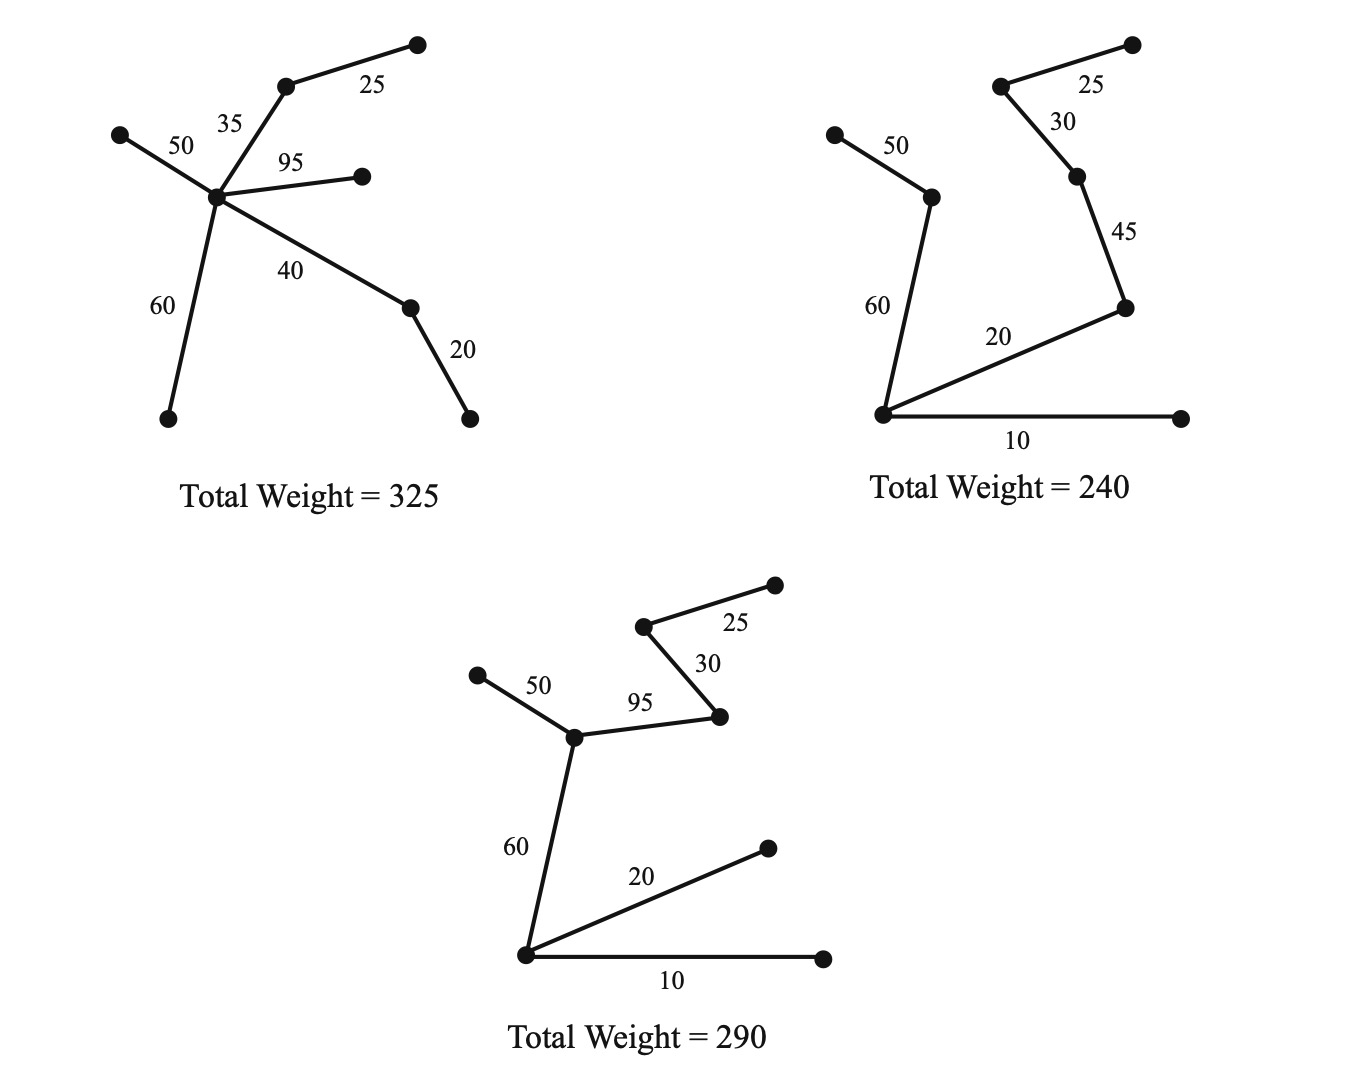
\includegraphics[height=5.8cm,width=0.95\textwidth,keepaspectratio]{figure_spanning_tree_examples.png}\par}
\vfill
{\tiny\raggedright Figure source: Harris, Hirst, and Mossinghoff, \emph{Combinatorics and Graph Theory}, 2nd ed., Springer, 2008, \S1.3.3, spanning trees of the city graph.\par}
\end{frame}

\begin{frame}{Kruskal's Algorithm}
\large
There are a number of fairly simple algorithms for finding minimum weight spanning trees. Perhaps the best known is Kruskal's algorithm.
\par\medskip
\begin{block}{Algorithm}
\begin{enumerate}
\setlength{\itemsep}{0.22cm}
\item Start with all vertices and no chosen edges.
\item Consider the edges in order of increasing weight.
\item Add an edge if it creates no cycle with the chosen edges. Otherwise skip it.
\item Stop after choosing $n-1$ edges.
\end{enumerate}
\end{block}
\par\medskip Ties may be resolved in any order. The chosen edges form a forest at every step.
\end{frame}

\begin{frame}[t]{Kruskal's Algorithm for the Railroad Problem}
\normalsize
\vspace{0.1cm}
\begin{center}
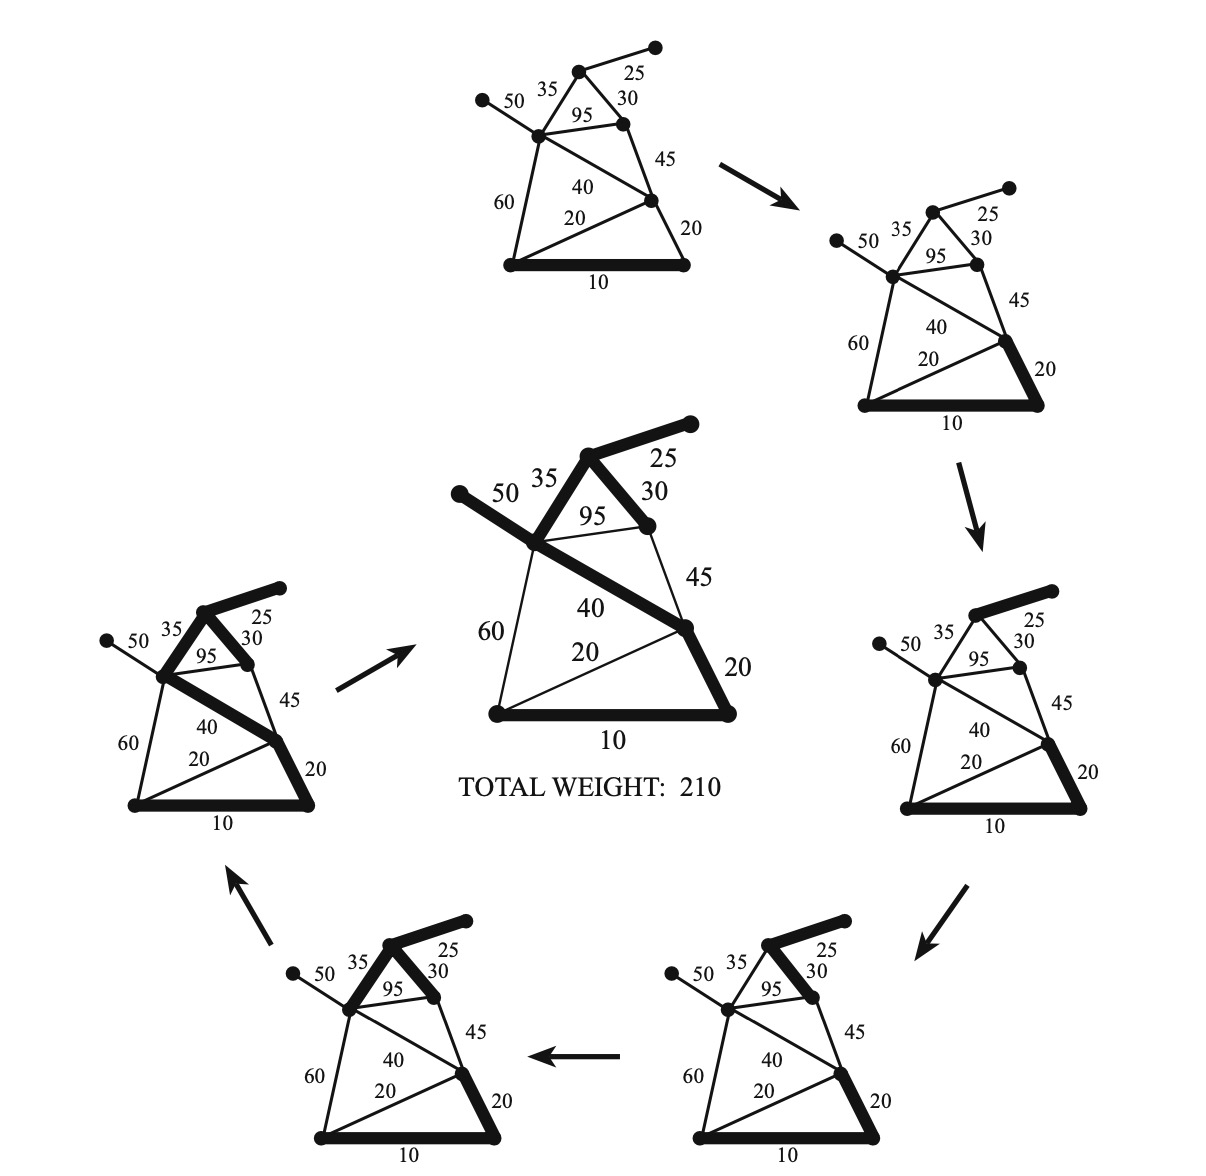
\includegraphics[height=6.3cm,width=0.96\textwidth,keepaspectratio]{figure_kruskal_railroad.png}
\end{center}
\vfill
{\tiny\raggedright Figure source: Harris, Hirst, and Mossinghoff, \emph{Combinatorics and Graph Theory}, 2nd ed., Springer, 2008, \S1.3.3, Kruskal's algorithm for the city graph.\par}
\end{frame}


\begin{frame}{Kruskal's Algorithm: Step 1}
\large
Choose $ab$ of weight $1$.\begin{center}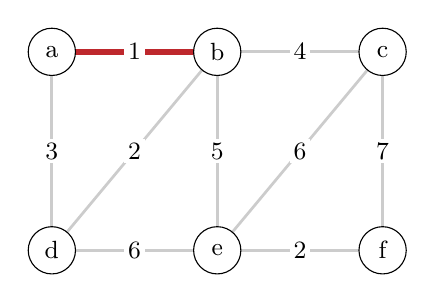
\begin{tikzpicture}[scale=1.05]
\coordinate (pa) at (0,1.4);
\coordinate (pb) at (2,1.4);
\coordinate (pc) at (4,1.4);
\coordinate (pd) at (0,-1);
\coordinate (pe) at (2,-1);
\coordinate (pf) at (4,-1);
\draw[selected] (pa) -- node[midway,fill=white,inner sep=1.4pt,font=\small,text=black]{1} (pb);
\draw[draw=black!20,line width=1pt] (pb) -- node[midway,fill=white,inner sep=1.4pt,font=\small,text=black]{4} (pc);
\draw[draw=black!20,line width=1pt] (pa) -- node[midway,fill=white,inner sep=1.4pt,font=\small,text=black]{3} (pd);
\draw[draw=black!20,line width=1pt] (pb) -- node[midway,fill=white,inner sep=1.4pt,font=\small,text=black]{5} (pe);
\draw[draw=black!20,line width=1pt] (pc) -- node[midway,fill=white,inner sep=1.4pt,font=\small,text=black]{7} (pf);
\draw[draw=black!20,line width=1pt] (pd) -- node[midway,fill=white,inner sep=1.4pt,font=\small,text=black]{6} (pe);
\draw[draw=black!20,line width=1pt] (pe) -- node[midway,fill=white,inner sep=1.4pt,font=\small,text=black]{2} (pf);
\draw[draw=black!20,line width=1pt] (pb) -- node[midway,fill=white,inner sep=1.4pt,font=\small,text=black]{2} (pd);
\draw[draw=black!20,line width=1pt] (pc) -- node[midway,fill=white,inner sep=1.4pt,font=\small,text=black]{6} (pe);
\node[lab] at (pa) {a};
\node[lab] at (pb) {b};
\node[lab] at (pc) {c};
\node[lab] at (pd) {d};
\node[lab] at (pe) {e};
\node[lab] at (pf) {f};
\end{tikzpicture}\end{center}\begin{center}Chosen edges are red. Total weight: $1$.\end{center}
\end{frame}

\begin{frame}{Kruskal's Algorithm: Step 2}
\large
Choose $bd$ of weight $2$.\begin{center}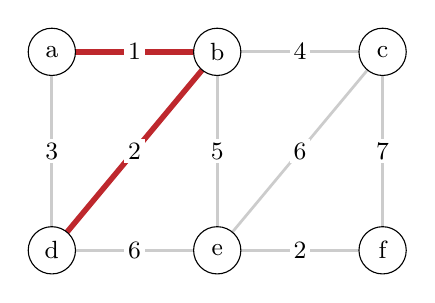
\begin{tikzpicture}[scale=1.05]
\coordinate (pa) at (0,1.4);
\coordinate (pb) at (2,1.4);
\coordinate (pc) at (4,1.4);
\coordinate (pd) at (0,-1);
\coordinate (pe) at (2,-1);
\coordinate (pf) at (4,-1);
\draw[selected] (pa) -- node[midway,fill=white,inner sep=1.4pt,font=\small,text=black]{1} (pb);
\draw[draw=black!20,line width=1pt] (pb) -- node[midway,fill=white,inner sep=1.4pt,font=\small,text=black]{4} (pc);
\draw[draw=black!20,line width=1pt] (pa) -- node[midway,fill=white,inner sep=1.4pt,font=\small,text=black]{3} (pd);
\draw[draw=black!20,line width=1pt] (pb) -- node[midway,fill=white,inner sep=1.4pt,font=\small,text=black]{5} (pe);
\draw[draw=black!20,line width=1pt] (pc) -- node[midway,fill=white,inner sep=1.4pt,font=\small,text=black]{7} (pf);
\draw[draw=black!20,line width=1pt] (pd) -- node[midway,fill=white,inner sep=1.4pt,font=\small,text=black]{6} (pe);
\draw[draw=black!20,line width=1pt] (pe) -- node[midway,fill=white,inner sep=1.4pt,font=\small,text=black]{2} (pf);
\draw[selected] (pb) -- node[midway,fill=white,inner sep=1.4pt,font=\small,text=black]{2} (pd);
\draw[draw=black!20,line width=1pt] (pc) -- node[midway,fill=white,inner sep=1.4pt,font=\small,text=black]{6} (pe);
\node[lab] at (pa) {a};
\node[lab] at (pb) {b};
\node[lab] at (pc) {c};
\node[lab] at (pd) {d};
\node[lab] at (pe) {e};
\node[lab] at (pf) {f};
\end{tikzpicture}\end{center}\begin{center}Chosen edges are red. Total weight: $3$.\end{center}
\end{frame}

\begin{frame}{Kruskal's Algorithm: Step 3}
\large
Choose $ef$ of weight $2$.\begin{center}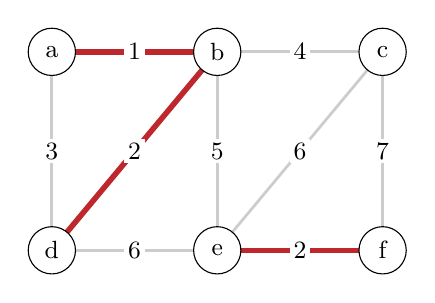
\begin{tikzpicture}[scale=1.05]
\coordinate (pa) at (0,1.4);
\coordinate (pb) at (2,1.4);
\coordinate (pc) at (4,1.4);
\coordinate (pd) at (0,-1);
\coordinate (pe) at (2,-1);
\coordinate (pf) at (4,-1);
\draw[selected] (pa) -- node[midway,fill=white,inner sep=1.4pt,font=\small,text=black]{1} (pb);
\draw[draw=black!20,line width=1pt] (pb) -- node[midway,fill=white,inner sep=1.4pt,font=\small,text=black]{4} (pc);
\draw[draw=black!20,line width=1pt] (pa) -- node[midway,fill=white,inner sep=1.4pt,font=\small,text=black]{3} (pd);
\draw[draw=black!20,line width=1pt] (pb) -- node[midway,fill=white,inner sep=1.4pt,font=\small,text=black]{5} (pe);
\draw[draw=black!20,line width=1pt] (pc) -- node[midway,fill=white,inner sep=1.4pt,font=\small,text=black]{7} (pf);
\draw[draw=black!20,line width=1pt] (pd) -- node[midway,fill=white,inner sep=1.4pt,font=\small,text=black]{6} (pe);
\draw[selected] (pe) -- node[midway,fill=white,inner sep=1.4pt,font=\small,text=black]{2} (pf);
\draw[selected] (pb) -- node[midway,fill=white,inner sep=1.4pt,font=\small,text=black]{2} (pd);
\draw[draw=black!20,line width=1pt] (pc) -- node[midway,fill=white,inner sep=1.4pt,font=\small,text=black]{6} (pe);
\node[lab] at (pa) {a};
\node[lab] at (pb) {b};
\node[lab] at (pc) {c};
\node[lab] at (pd) {d};
\node[lab] at (pe) {e};
\node[lab] at (pf) {f};
\end{tikzpicture}\end{center}\begin{center}Chosen edges are red. Total weight: $5$.\end{center}
\end{frame}

\begin{frame}{Kruskal's Algorithm: Step 4}
\large
Skip $ad$ of weight $3$: it closes a cycle. Choose $bc$ of weight $4$.\begin{center}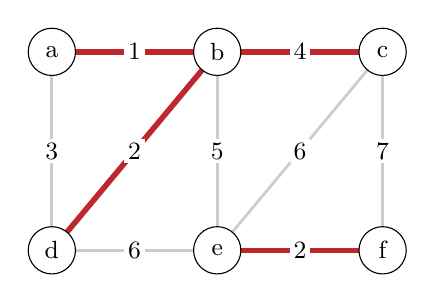
\begin{tikzpicture}[scale=1.05]
\coordinate (pa) at (0,1.4);
\coordinate (pb) at (2,1.4);
\coordinate (pc) at (4,1.4);
\coordinate (pd) at (0,-1);
\coordinate (pe) at (2,-1);
\coordinate (pf) at (4,-1);
\draw[selected] (pa) -- node[midway,fill=white,inner sep=1.4pt,font=\small,text=black]{1} (pb);
\draw[selected] (pb) -- node[midway,fill=white,inner sep=1.4pt,font=\small,text=black]{4} (pc);
\draw[draw=black!20,line width=1pt] (pa) -- node[midway,fill=white,inner sep=1.4pt,font=\small,text=black]{3} (pd);
\draw[draw=black!20,line width=1pt] (pb) -- node[midway,fill=white,inner sep=1.4pt,font=\small,text=black]{5} (pe);
\draw[draw=black!20,line width=1pt] (pc) -- node[midway,fill=white,inner sep=1.4pt,font=\small,text=black]{7} (pf);
\draw[draw=black!20,line width=1pt] (pd) -- node[midway,fill=white,inner sep=1.4pt,font=\small,text=black]{6} (pe);
\draw[selected] (pe) -- node[midway,fill=white,inner sep=1.4pt,font=\small,text=black]{2} (pf);
\draw[selected] (pb) -- node[midway,fill=white,inner sep=1.4pt,font=\small,text=black]{2} (pd);
\draw[draw=black!20,line width=1pt] (pc) -- node[midway,fill=white,inner sep=1.4pt,font=\small,text=black]{6} (pe);
\node[lab] at (pa) {a};
\node[lab] at (pb) {b};
\node[lab] at (pc) {c};
\node[lab] at (pd) {d};
\node[lab] at (pe) {e};
\node[lab] at (pf) {f};
\end{tikzpicture}\end{center}\begin{center}Chosen edges are red. Total weight: $9$.\end{center}
\end{frame}

\begin{frame}{Kruskal's Algorithm: Step 5}
\large
Choose $be$ of weight $5$. All six vertices are now connected.\begin{center}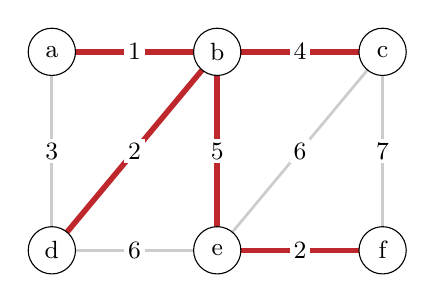
\begin{tikzpicture}[scale=1.05]
\coordinate (pa) at (0,1.4);
\coordinate (pb) at (2,1.4);
\coordinate (pc) at (4,1.4);
\coordinate (pd) at (0,-1);
\coordinate (pe) at (2,-1);
\coordinate (pf) at (4,-1);
\draw[selected] (pa) -- node[midway,fill=white,inner sep=1.4pt,font=\small,text=black]{1} (pb);
\draw[selected] (pb) -- node[midway,fill=white,inner sep=1.4pt,font=\small,text=black]{4} (pc);
\draw[draw=black!20,line width=1pt] (pa) -- node[midway,fill=white,inner sep=1.4pt,font=\small,text=black]{3} (pd);
\draw[selected] (pb) -- node[midway,fill=white,inner sep=1.4pt,font=\small,text=black]{5} (pe);
\draw[draw=black!20,line width=1pt] (pc) -- node[midway,fill=white,inner sep=1.4pt,font=\small,text=black]{7} (pf);
\draw[draw=black!20,line width=1pt] (pd) -- node[midway,fill=white,inner sep=1.4pt,font=\small,text=black]{6} (pe);
\draw[selected] (pe) -- node[midway,fill=white,inner sep=1.4pt,font=\small,text=black]{2} (pf);
\draw[selected] (pb) -- node[midway,fill=white,inner sep=1.4pt,font=\small,text=black]{2} (pd);
\draw[draw=black!20,line width=1pt] (pc) -- node[midway,fill=white,inner sep=1.4pt,font=\small,text=black]{6} (pe);
\node[lab] at (pa) {a};
\node[lab] at (pb) {b};
\node[lab] at (pc) {c};
\node[lab] at (pd) {d};
\node[lab] at (pe) {e};
\node[lab] at (pf) {f};
\end{tikzpicture}\end{center}\begin{center}Chosen edges are red. Total weight: $14$.\end{center}
\end{frame}

\begin{frame}{Why Does Kruskal's Algorithm Produce a Tree?}
\large
\begin{enumerate}
\setlength{\itemsep}{0.22cm}
\item An edge is added only when it joins two different components, so no cycle is ever formed.
\item If the chosen forest were still disconnected after all edges had been considered, connectedness of $G$ would provide an edge between two components. That edge could not have been skipped.
\item Thus the algorithm reaches a connected forest: a spanning tree.
\end{enumerate}\par\medskip But why must its total weight be minimum?
\end{frame}

\begin{frame}[t]{Theorem: Kruskal's Algorithm Is Optimal}
\large
\begin{block}{Theorem 1.17}
Kruskal's algorithm produces a minimum weight spanning tree.
\end{block}
\end{frame}

\begin{frame}[t]{Theorem: Kruskal's Algorithm Is Optimal}
\large
\begin{block}{Theorem 1.17}
Kruskal's algorithm produces a minimum weight spanning tree.
\end{block}
\begin{block}{Proof}
\normalsize
Assume $G$ is connected. Let $T$ be the spanning tree produced by Kruskal's algorithm, with edges $e_1,\ldots,e_{n-1}$ listed in the order chosen.
\par\medskip
Among all minimum weight spanning trees of $G$, choose $T'$ that agrees with $T$ for as long as possible: the initial sequence $e_1,\ldots,e_k$ contained in $T'$ is as long as possible.
\par\medskip
If $T'=T$, we are done. Otherwise, $0\le k<n-1$ and
\[
e_1,\ldots,e_k\in E(T'),\qquad e_{k+1}\notin E(T').
\]
\end{block}
\end{frame}

\begin{frame}[t]{Proof continued}
\begin{block}{Proof of Theorem 1.17 (continued)}
\small
Adding $e_{k+1}$ to $T'$ creates a unique cycle $C$. Since $e_1,\ldots,e_k,e_{k+1}$ form a forest, $C$ contains another edge $f\in E(T')$ joining different components of the forest $F=\{e_1,\ldots,e_k\}$. In particular, $f\notin F$.
\par\smallskip
The edge $f$ was eligible when Kruskal chose $e_{k+1}$, so $w(e_{k+1})\le w(f)$. Replacing $f$ by $e_{k+1}$ gives a spanning tree
\[
T''=T'+e_{k+1}-f,\qquad w(T'')=w(T')+w(e_{k+1})-w(f)\le w(T').
\]
Thus $T''$ is also minimum, but contains $e_1,\ldots,e_k,e_{k+1}$, contradicting the choice of $T'$. Hence $T$ is a minimum weight spanning tree.\hfill$\square$
\end{block}
\smallskip
{\centering
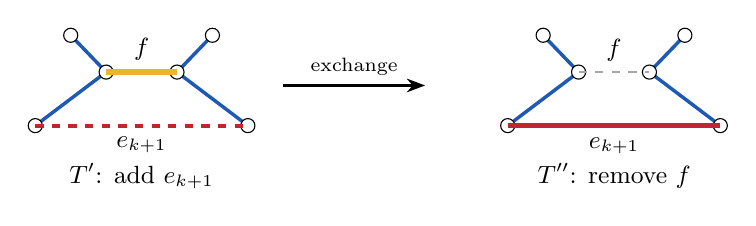
\begin{tikzpicture}[x=0.9cm,y=0.85cm]
\foreach \shift/\tag in {0/L,6/R} {
\begin{scope}[xshift=\shift cm]
\coordinate (\tag a) at (0,0); \coordinate (\tag b) at (1,0.8);
\coordinate (\tag c) at (2,0.8); \coordinate (\tag d) at (3,0);
\coordinate (\tag x) at (.5,1.35); \coordinate (\tag y) at (2.5,1.35);
\foreach \u/\v in {a/b,c/d,b/x,c/y} \draw[edge] (\tag\u)--(\tag\v);
\foreach \v in {a,b,c,d,x,y} \node[v] at (\tag\v) {};
\end{scope}}
\draw[draw=MapGold,line width=2pt] (Lb)--node[above,font=\small,text=black]{$f$}(Lc);
\draw[draw=RamRed,line width=1.5pt,dashed] (La)--node[below,font=\small]{$e_{k+1}$}(Ld);
\draw[draw=black!35,dashed,line width=1pt] (Rb)--node[above,font=\small,text=black]{$f$}(Rc);
\draw[draw=RamRed,line width=2pt] (Ra)--node[below,font=\small]{$e_{k+1}$}(Rd);
\draw[-{Stealth},thick] (3.5,.6)--node[above,font=\scriptsize]{exchange}(5.5,.6);
\node[font=\small] at (1.5,-.75) {$T'$: add $e_{k+1}$};
\node[font=\small] at (8.17,-.75) {$T''$: remove $f$};
\end{tikzpicture}\par}
\end{frame}


\begin{frame}{Another Algorithm: Prim's Algorithm}
\normalsize
\begin{block}{Algorithm}
\begin{enumerate}
\setlength{\itemsep}{0.22cm}
\item Start at any vertex.
\item Choose a cheapest edge joining a reached vertex to an unreached vertex.
\item Add the edge and the new vertex. Repeat until every vertex is reached.
\end{enumerate}
\end{block}
\par\medskip Kruskal grows a forest. Prim grows one connected tree.\par\medskip\textbf{Exercise.} Apply Prim starting at $a$ in our six-town example.
\end{frame}

\section{Counting Trees}
\begin{frame}{Counting Trees: Labels Matter}
\large
\begin{block}{Labeled trees}
The vertex labels are fixed. Changing which labeled vertices are joined can give a different tree, even if the two trees are isomorphic.
\end{block}
\begin{center}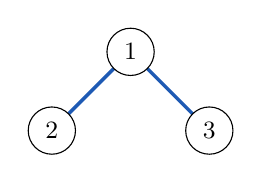
\begin{tikzpicture}[scale=1]
\coordinate (p1) at (0,1);
\coordinate (p2) at (-1,0);
\coordinate (p3) at (1,0);
\draw[edge] (p1) -- (p2);
\draw[edge] (p1) -- (p3);
\node[lab] at (p1) {1};
\node[lab] at (p2) {2};
\node[lab] at (p3) {3};
\end{tikzpicture}\qquad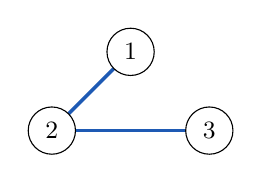
\begin{tikzpicture}[scale=1]
\coordinate (p1) at (0,1);
\coordinate (p2) at (-1,0);
\coordinate (p3) at (1,0);
\draw[edge] (p1) -- (p2);
\draw[edge] (p2) -- (p3);
\node[lab] at (p1) {1};
\node[lab] at (p2) {2};
\node[lab] at (p3) {3};
\end{tikzpicture}\qquad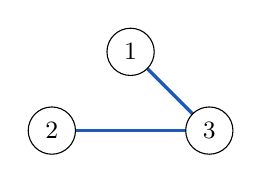
\begin{tikzpicture}[scale=1]
\coordinate (p1) at (0,1);
\coordinate (p2) at (-1,0);
\coordinate (p3) at (1,0);
\draw[edge] (p1) -- (p3);
\draw[edge] (p2) -- (p3);
\node[lab] at (p1) {1};
\node[lab] at (p2) {2};
\node[lab] at (p3) {3};
\end{tikzpicture}\end{center}\begin{center}Three labeled trees on $\{1,2,3\}$, but only one shape.\end{center}
\end{frame}

\begin{frame}{Theorem: Cayley's Tree Formula}
\large
How many different trees can we form on $n$ vertices with fixed labels? We count trees as different when their edges join different pairs of labels, even if their shapes are the same. Cayley's formula gives this number directly.
\par\medskip
\begin{block}{Theorem 1.18 (Cayley's Tree Formula)}
There are $n^{n-2}$ distinct labeled trees of order $n$.
\end{block}
\begin{center}\begin{tabular}{c|rrrrr}$n$&2&3&4&5&6\\\hline Trees&1&3&16&125&1296\end{tabular}\end{center}\par\medskip The case $n=1$ has one tree, $K_1$.\par\medskip\normalsize
\textbf{Proof idea.} We prove the formula by establishing a one-to-one correspondence between labeled trees on $\{1,\ldots,n\}$ and sequences of length $n-2$ with entries in $\{1,\ldots,n\}$. There are $n^{n-2}$ such sequences, so there are $n^{n-2}$ labeled trees.
\par\smallskip
The following slides present the two algorithms for going back and forth: from a tree to its sequence, and from a sequence to its unique tree.
\end{frame}

\begin{frame}{Pr\"ufer's Method for Assigning a Sequence to a Labeled Tree}
\normalsize
This algorithm assigns each labeled tree a sequence of length $n-2$: each step records one label and removes one vertex, stopping when two vertices remain.
\par\medskip
\begin{block}{Algorithm}
\textbf{Given:} A tree $T$, with vertices labeled $1,\ldots,n$.
\par\medskip
\begin{enumerate}
\setlength{\itemsep}{0.22cm}
\item Let $i=0$, and let $T_0=T$.
\item Find the leaf on $T_i$ with the smallest label and call it $v$.
\item Record in the sequence the label of $v$'s neighbor.
\item Remove $v$ from $T_i$ to create a new tree $T_{i+1}$.
\item If $T_{i+1}=K_2$, then stop. Otherwise, increment $i$ by $1$ and go back to step $2$.
\end{enumerate}
\end{block}
\end{frame}

\begin{frame}{Pr\"ufer Example: Step 1}
\large
\begin{center}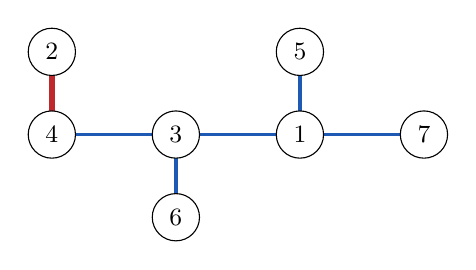
\begin{tikzpicture}[scale=1.05]
\coordinate (p1) at (0,0);
\coordinate (p2) at (-3,1);
\coordinate (p3) at (-1.5,0);
\coordinate (p4) at (-3,0);
\coordinate (p5) at (0,1);
\coordinate (p6) at (-1.5,-1);
\coordinate (p7) at (1.5,0);
\draw[selected] (p2) -- (p4);
\draw[edge] (p4) -- (p3);
\draw[edge] (p3) -- (p1);
\draw[edge] (p1) -- (p5);
\draw[edge] (p3) -- (p6);
\draw[edge] (p1) -- (p7);
\node[lab] at (p1) {1};
\node[lab] at (p2) {2};
\node[lab] at (p3) {3};
\node[lab] at (p4) {4};
\node[lab] at (p5) {5};
\node[lab] at (p6) {6};
\node[lab] at (p7) {7};
\end{tikzpicture}\end{center}\par\medskip Smallest leaf: $2$. Record its neighbor: $4$.\begin{block}{Sequence so far}
\[4\]
\end{block}

\end{frame}

\begin{frame}{Pr\"ufer Example: Step 2}
\large
\begin{center}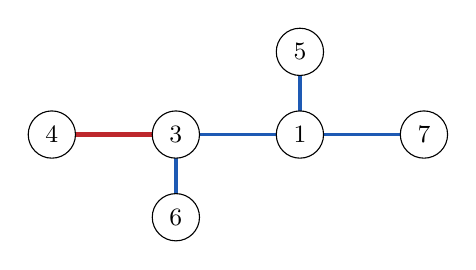
\begin{tikzpicture}[scale=1.05]
\coordinate (p1) at (0,0);
\coordinate (p3) at (-1.5,0);
\coordinate (p4) at (-3,0);
\coordinate (p5) at (0,1);
\coordinate (p6) at (-1.5,-1);
\coordinate (p7) at (1.5,0);
\draw[selected] (p4) -- (p3);
\draw[edge] (p3) -- (p1);
\draw[edge] (p1) -- (p5);
\draw[edge] (p3) -- (p6);
\draw[edge] (p1) -- (p7);
\node[lab] at (p1) {1};
\node[lab] at (p3) {3};
\node[lab] at (p4) {4};
\node[lab] at (p5) {5};
\node[lab] at (p6) {6};
\node[lab] at (p7) {7};
\end{tikzpicture}\end{center}\par\medskip Smallest leaf: $4$. Record its neighbor: $3$.\begin{block}{Sequence so far}
\[4,3\]
\end{block}

\end{frame}

\begin{frame}{Pr\"ufer Example: Step 3}
\large
\begin{center}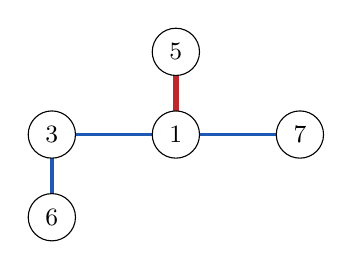
\begin{tikzpicture}[scale=1.05]
\coordinate (p1) at (0,0);
\coordinate (p3) at (-1.5,0);
\coordinate (p5) at (0,1);
\coordinate (p6) at (-1.5,-1);
\coordinate (p7) at (1.5,0);
\draw[edge] (p3) -- (p1);
\draw[selected] (p1) -- (p5);
\draw[edge] (p3) -- (p6);
\draw[edge] (p1) -- (p7);
\node[lab] at (p1) {1};
\node[lab] at (p3) {3};
\node[lab] at (p5) {5};
\node[lab] at (p6) {6};
\node[lab] at (p7) {7};
\end{tikzpicture}\end{center}\par\medskip Smallest leaf: $5$. Record its neighbor: $1$.\begin{block}{Sequence so far}
\[4,3,1\]
\end{block}

\end{frame}

\begin{frame}{Pr\"ufer Example: Step 4}
\large
\begin{center}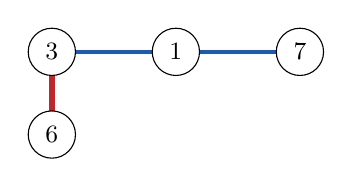
\begin{tikzpicture}[scale=1.05]
\coordinate (p1) at (0,0);
\coordinate (p3) at (-1.5,0);
\coordinate (p6) at (-1.5,-1);
\coordinate (p7) at (1.5,0);
\draw[edge] (p3) -- (p1);
\draw[selected] (p3) -- (p6);
\draw[edge] (p1) -- (p7);
\node[lab] at (p1) {1};
\node[lab] at (p3) {3};
\node[lab] at (p6) {6};
\node[lab] at (p7) {7};
\end{tikzpicture}\end{center}\par\medskip Smallest leaf: $6$. Record its neighbor: $3$.\begin{block}{Sequence so far}
\[4,3,1,3\]
\end{block}

\end{frame}

\begin{frame}{Pr\"ufer Example: Step 5}
\large
\begin{center}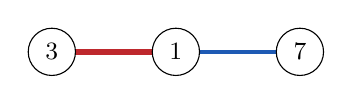
\begin{tikzpicture}[scale=1.05]
\coordinate (p1) at (0,0);
\coordinate (p3) at (-1.5,0);
\coordinate (p7) at (1.5,0);
\draw[selected] (p3) -- (p1);
\draw[edge] (p1) -- (p7);
\node[lab] at (p1) {1};
\node[lab] at (p3) {3};
\node[lab] at (p7) {7};
\end{tikzpicture}\end{center}\par\medskip Smallest leaf: $3$. Record its neighbor: $1$.\begin{block}{Sequence so far}
\[4,3,1,3,1\]
\end{block}

\end{frame}

\begin{frame}{What Does the Pr\"ufer Sequence Remember?}
\large
\begin{block}{Degree formula}
For every vertex $v$,\[\deg_T(v)=1+\#\{\text{occurrences of }v\text{ in the sequence}\}.\]
\end{block}
Each recorded occurrence removes one edge incident to $v$. Exactly one incident edge remains when $v$ is deleted or reaches the final pair.\par\bigskip\textbf{Consequently:} the leaves are exactly the labels absent from the sequence.
\end{frame}

\begin{frame}{Pr\"ufer's Method for Constructing a Tree from a Sequence}
\normalsize
We can reverse the procedure: every sequence of length $n-2$ with entries in $\{1,\ldots,n\}$ determines a unique labeled tree. The algorithm below reconstructs that tree, undoing the leaf-removal process.
\par\medskip
\begin{block}{Algorithm}
\textbf{Given:} A sequence $(a_1,\ldots,a_{n-2})$, with each $a_i\in\{1,\ldots,n\}$.
\par\smallskip
\begin{enumerate}
\setlength{\itemsep}{0.16cm}
\item Start with vertices labeled $1,\ldots,n$, no edges, and $S=\{1,\ldots,n\}$.
\item Find the smallest label $b\in S$ that does not occur in the remaining sequence.
\item Join $b$ to the vertex whose label is the first entry of the sequence.
\item Remove $b$ from $S$ and delete the first entry. If entries remain, return to step $2$.
\item Join the two remaining vertices in $S$.
\end{enumerate}
\end{block}
\par\smallskip For $n=2$, the sequence is empty: simply join vertices $1$ and $2$.
\end{frame}

\begin{frame}{Decoding $(4,3,1,3,1)$}
\normalsize
\begin{center}\renewcommand{\arraystretch}{1.3}\begin{tabular}{c|c|c|c}Remaining sequence&Smallest absent label&Add edge&Remove label\\\hline
$(4,3,1,3,1)$&2&$24$&2\\$(3,1,3,1)$&4&$43$&4\\$(1,3,1)$&5&$51$&5\\$(3,1)$&6&$63$&6\\$(1)$&3&$31$&3\\empty&$1,7$ remain&$17$&---\end{tabular}\end{center}\begin{center}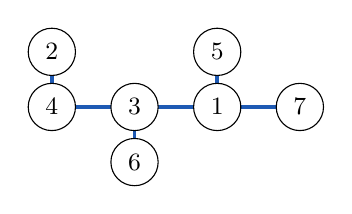
\begin{tikzpicture}[scale=0.7]
\coordinate (p1) at (0,0);
\coordinate (p2) at (-3,1);
\coordinate (p3) at (-1.5,0);
\coordinate (p4) at (-3,0);
\coordinate (p5) at (0,1);
\coordinate (p6) at (-1.5,-1);
\coordinate (p7) at (1.5,0);
\draw[edge] (p2) -- (p4);
\draw[edge] (p4) -- (p3);
\draw[edge] (p3) -- (p1);
\draw[edge] (p1) -- (p5);
\draw[edge] (p3) -- (p6);
\draw[edge] (p1) -- (p7);
\node[lab] at (p1) {1};
\node[lab] at (p2) {2};
\node[lab] at (p3) {3};
\node[lab] at (p4) {4};
\node[lab] at (p5) {5};
\node[lab] at (p6) {6};
\node[lab] at (p7) {7};
\end{tikzpicture}\end{center}
\end{frame}

\begin{frame}{Proof of Cayley's Formula}
\normalsize
\begin{enumerate}
\setlength{\itemsep}{0.22cm}
\item Decoding any sequence produces a tree: read the construction backward, starting with the final edge and attaching one new leaf at each step.
\item In each remaining tree, its leaves are precisely the remaining labels absent from the remaining sequence. Thus encoding and decoding select the same smallest leaf and the same neighbor.
\item The procedures are inverse, so trees correspond bijectively to sequences in $\{1,\ldots,n\}^{n-2}$.
\end{enumerate}\[\#\text{trees}=\underbrace{n\cdot n\cdots n}_{n-2\text{ entries}}=n^{n-2}.\qquad\square\]
\end{frame}

\begin{frame}{Questions About Pr\"ufer Sequences}
\large
\begin{enumerate}
\setlength{\itemsep}{0.22cm}
\item Which tree corresponds to the constant sequence $(a,a,\ldots,a)$?
\item What can you say about a tree whose sequence entries are all distinct?
\item How many labeled trees on $n\ge3$ vertices have vertex $1$ as a leaf?
\end{enumerate}
\end{frame}

\begin{frame}{Questions About Pr\"ufer Sequences: Answers}
\large
\begin{enumerate}
\setlength{\itemsep}{0.22cm}
\item A star with center $a$. Its center has degree $n-1$, and all other degrees are $1$.
\item Every degree is at most $2$, so the tree is a path.
\item The sequence must avoid $1$. Each of its $n-2$ entries has $n-1$ choices, giving $(n-1)^{n-2}$ trees.
\end{enumerate}
\end{frame}

\begin{frame}{Counting Spanning Trees: Toward the Matrix Tree Theorem}
\large
Cayley's formula counts labeled trees on $n$ vertices. Equivalently, it counts the spanning trees of the complete graph $K_n$.
\par\bigskip
What if the graph is not complete? We would like a way to count spanning trees when only certain pairs of vertices are joined by edges.
\par\bigskip
The \textbf{Matrix Tree Theorem} answers this more general question. Proved by Kirchhoff in 1847, it connects the number of spanning trees of a graph to a determinant formed from its matrices.
\end{frame}

\begin{frame}[t]{Definitions: Degree Matrix and Cofactor}
\normalsize
To state the Matrix Tree Theorem, we need two definitions. Recall that $A$ denotes the adjacency matrix.
\begin{block}{Degree matrix}
For vertices $v_1,\ldots,v_n$, define the $n\times n$ matrix $D$ by
\[
[D]_{i,j}=\begin{cases}\deg(v_i),&i=j,\\0,&i\ne j.\end{cases}
\]
Thus $D$ lists the vertex degrees on its diagonal and is zero elsewhere.
\end{block}
\begin{block}{Cofactor}
For an $n\times n$ matrix $B$, its $(i,j)$ cofactor is $(-1)^{i+j}\det B(i\mid j)$, where $B(i\mid j)$ is obtained by deleting row $i$ and column $j$.
\end{block}
\end{frame}

\begin{frame}[t]{Theorem: The Matrix Tree Theorem}
\normalsize
\large
\begin{block}{Theorem 1.19 (Matrix Tree Theorem)}
For a connected labeled graph $G$, let $A$ be its adjacency matrix and $D$ its degree matrix. Every cofactor of $D-A$ equals the number of spanning trees of $G$.
\end{block}
\end{frame}

\begin{frame}[t]{Matrix Tree Theorem: The Proof in Three Steps}
Fix a vertex $v_r$, called the \textbf{root}. We first count trees using the $(r,r)$ cofactor.
\begin{block}{The plan}
\begin{enumerate}
\item Write the matrix with row and column $r$ deleted as $BB^{\mathsf T}$, using a signed incidence matrix.
\medskip
\item Expand $\det(BB^{\mathsf T})$ as a sum over sets of $n-1$ edges.
\medskip
\item Show that each spanning tree contributes $1$, and every other edge set contributes $0$.
\end{enumerate}
\end{block}
\medskip
Finally, we explain why all cofactors have the same value.
\end{frame}

\begin{frame}[t]{Step 1: Give Each Edge a Direction}
Let $G$ have $n$ vertices and $m$ edges. Choose a direction for each edge; these directions are only a bookkeeping device.
\begin{block}{Signed incidence matrix $M$}
The column for an edge $u\longrightarrow v$ has $-1$ in row $u$, $+1$ in row $v$, and zeros elsewhere.
\end{block}
\begin{columns}[c,onlytextwidth]
\begin{column}{.42\textwidth}
\centering
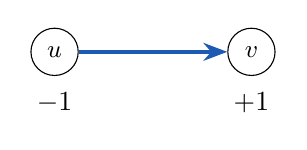
\begin{tikzpicture}
\node[lab] (u) at (0,0) {$u$};\node[lab] (v) at (2.5,0) {$v$};
\draw[edge,-{Stealth}] (u)--(v);
\node at (0,-.65) {$-1$};\node at (2.5,-.65) {$+1$};
\end{tikzpicture}
\end{column}
\begin{column}{.54\textwidth}
Thus $M$ is $n\times m$. Reversing an edge multiplies its column by $-1$.
\end{column}
\end{columns}
\end{frame}

\begin{frame}[t]{Step 1: Recovering the Degree and Adjacency Matrices}
\begin{block}{Claim A}
\[MM^{\mathsf T}=D-A.\]
\end{block}
\begin{block}{Proof: take dot products of rows}
\textbf{Diagonal entry:} row $i$ has one entry $\pm1$ for each edge at $v_i$. Its squared length is $\deg(v_i)$.
\par\medskip
\textbf{Off-diagonal entry:} rows $i$ and $j$ overlap only in a column for an edge joining $v_i$ and $v_j$. That column contributes $(-1)(+1)=-1$.
\par\medskip
Hence the diagonal entries are those of $D$, and the off-diagonal entries are those of $-A$.
\end{block}
\end{frame}

\begin{frame}[t]{Step 1: Delete the Root Row}
Delete row $r$ of $M$ to obtain the $(n-1)\times m$ matrix $B$.
\begin{block}{The cofactor we want}
Deleting row and column $r$ of $MM^{\mathsf T}$ leaves the dot products of the remaining rows. Therefore
\[
(D-A)(r\mid r)=BB^{\mathsf T}.
\]
The $(r,r)$ cofactor is consequently $\det(BB^{\mathsf T})$.
\end{block}
\medskip
For $S\subseteq E(G)$ with $|S|=n-1$, write $B_S$ for the square matrix obtained by keeping the columns indexed by $S$.
\end{frame}

\begin{frame}[t]{Step 2: Expand the Determinant by Edge Sets}
\begin{block}{Cauchy--Binet formula}
For a $q\times m$ matrix $X$ and an $m\times q$ matrix $Y$,
\[
\det(XY)=\sum_{|S|=q}\det(X_{[:,S]})\det(Y_{[S,:]}).
\]
The sum runs over sets of $q$ column indices, in increasing order.
\end{block}
Apply this with $X=B$, $Y=B^{\mathsf T}$ and $q=n-1$:
\[
\boxed{\det(BB^{\mathsf T})=
\sum_{\substack{S\subseteq E(G)\\|S|=n-1}}(\det B_S)^2.}
\]
Each term now corresponds to a spanning subgraph with $n-1$ edges.
\end{frame}

\begin{frame}[t]{Step 3: Which Edge Sets Contribute?}
\begin{block}{Claim B}
For $H=(V(G),S)$ with $|S|=n-1$,
\[
(\det B_S)^2=
\begin{cases}
1,&H\text{ is a spanning tree},\\
0,&H\text{ is not a spanning tree}.
\end{cases}
\]
\end{block}
\medskip
\textbf{Tree:} remove a leaf other than the root and expand the determinant along its row.
\par\bigskip
\textbf{Not a tree:} find a component not containing the root; its rows sum to zero.
\end{frame}

\begin{frame}[t]{Claim B: A Tree Contributes One}
\begin{block}{Proof by removing leaves}
If $H$ is a tree with at least two vertices, choose a leaf $u\ne v_r$ and let $e$ be its only edge.
\par\medskip
The row of $B_S$ for $u$ has just one nonzero entry, equal to $\pm1$, in column $e$. Expanding along this row gives
\[
|\det B_S|=|\det B_{\mathrm{smaller\ tree}}|.
\]
The smaller matrix is the signed incidence matrix of $H-u$, with the same root row deleted. Repeat until only the root remains; the empty determinant is $1$.
\end{block}
\begin{center}
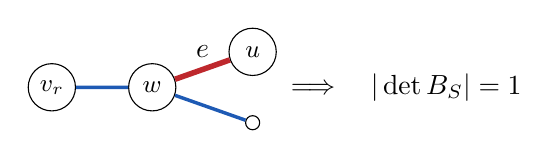
\begin{tikzpicture}[scale=.75]
\node[lab] (r) at (0,0) {$v_r$};\node[lab] (w) at (1.7,0) {$w$};\node[lab] (u) at (3.4,.6) {$u$};\node[v] (x) at (3.4,-.6) {};
\draw[edge] (r)--(w)--(x);\draw[selected] (w)--node[above] {$e$}(u);
\node at (6,0) {$\Longrightarrow\quad |\det B_S|=1$};
\end{tikzpicture}
\end{center}
\end{frame}

\begin{frame}[t]{Claim B: Every Other Edge Set Contributes Zero}
\begin{block}{Proof by finding dependent rows}
An $n$-vertex graph with $n-1$ edges is a tree if it is connected. Thus, if $H$ is not a tree, it is disconnected.
\par\medskip
Choose a component $C$ not containing $v_r$. All of its vertex rows remain in $B_S$.
\par\medskip
Sum these rows. An edge in $C$ contributes $-1+1=0$; an edge outside $C$ contributes $0$. No edge of $H$ leaves $C$.
\par\medskip
The sum is the zero row, so the rows are dependent and $\det B_S=0$.
\end{block}
\medskip
This also covers an isolated vertex: its row is already zero.
\end{frame}

\begin{frame}[t]{Putting the Pieces Together}
\begin{block}{The diagonal cofactor counts spanning trees}
\begin{align*}
\det((D-A)(r\mid r))
&=\det(BB^{\mathsf T})\\[.4em]
&=\sum_{\substack{S\subseteq E(G)\\|S|=n-1}}(\det B_S)^2\\[.4em]
&=\sum_{\substack{S\subseteq E(G)\\(V(G),S)\text{ is a tree}}}1.
\end{align*}
\end{block}
Every spanning tree has exactly $n-1$ edges and appears once.
\par\medskip
The root $v_r$ was arbitrary, so this proves the result for every diagonal cofactor.
\end{frame}

\begin{frame}[t]{Why Every Cofactor Has the Same Value}
\small
Set $L=D-A$ and $\mathbf1=(1,\ldots,1)^{\mathsf T}$. Since $L\mathbf1=0$, we have $\det L=0$.
\begin{block}{The only vectors in the kernel are constant}
If $Lx=0$, then
\[
0=x^{\mathsf T}Lx=\|M^{\mathsf T}x\|^2
=\sum_{uv\in E(G)}(x_u-x_v)^2.
\]
Thus $x_u=x_v$ along every edge. Connectedness implies $x$ is constant.
\end{block}
\begin{block}{Apply the cofactor identity}
Let $C_{ij}$ be the $(i,j)$ cofactor and let $Q_{ij}=C_{ji}$, the adjugate. Cofactor expansion gives
\[LQ=(\det L)I=0.\]
Each column of $Q$ is therefore constant. Its $j$th entry is $Q_{jj}=C_{jj}$, which we proved equals the number of spanning trees. Hence every entry of $Q$, and every cofactor, equals this number.\hfill$\square$
\end{block}
\end{frame}

\begin{frame}{Matrix Tree Theorem: An Example}
\normalsize
\begin{columns}[c,onlytextwidth]\begin{column}{.48\textwidth}\begin{center}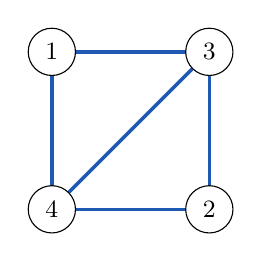
\begin{tikzpicture}[scale=1]
\coordinate (p1) at (-1,1);
\coordinate (p2) at (1,-1);
\coordinate (p3) at (1,1);
\coordinate (p4) at (-1,-1);
\draw[edge] (p1) -- (p3);
\draw[edge] (p1) -- (p4);
\draw[edge] (p2) -- (p3);
\draw[edge] (p2) -- (p4);
\draw[edge] (p3) -- (p4);
\node[lab] at (p1) {1};
\node[lab] at (p2) {2};
\node[lab] at (p3) {3};
\node[lab] at (p4) {4};
\end{tikzpicture}\end{center}\end{column}\begin{column}{.48\textwidth}\[D=\begin{pmatrix}2&0&0&0\\0&2&0&0\\0&0&3&0\\0&0&0&3\end{pmatrix}\]\[A=\begin{pmatrix}0&0&1&1\\0&0&1&1\\1&1&0&1\\1&1&1&0\end{pmatrix}\]\end{column}\end{columns}\begin{center}Vertex order: $1,2,3,4$.\end{center}
\end{frame}

\begin{frame}{Matrix Tree Theorem: Computing the Answer}
\large
\[D-A=\begin{pmatrix}2&0&-1&-1\\0&2&-1&-1\\-1&-1&3&-1\\-1&-1&-1&3\end{pmatrix}.\]Delete row $1$ and column $1$:\[\#\{\text{spanning trees of }G\}=\det\begin{pmatrix}2&-1&-1\\-1&3&-1\\-1&-1&3\end{pmatrix}=16-4-4=\boxed{8}.\]
\end{frame}

\begin{frame}{The Eight Spanning Trees}
\large
\begin{center}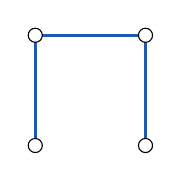
\begin{tikzpicture}[scale=0.7]
\coordinate (p1) at (-1,1);
\coordinate (p2) at (1,-1);
\coordinate (p3) at (1,1);
\coordinate (p4) at (-1,-1);
\draw[edge] (p1) -- (p3);
\draw[edge] (p1) -- (p4);
\draw[edge] (p2) -- (p3);
\node[v] at (p1) {};
\node[v] at (p2) {};
\node[v] at (p3) {};
\node[v] at (p4) {};
\end{tikzpicture}\qquad 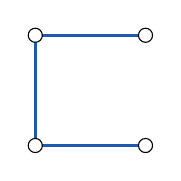
\begin{tikzpicture}[scale=0.7]
\coordinate (p1) at (-1,1);
\coordinate (p2) at (1,-1);
\coordinate (p3) at (1,1);
\coordinate (p4) at (-1,-1);
\draw[edge] (p1) -- (p3);
\draw[edge] (p1) -- (p4);
\draw[edge] (p2) -- (p4);
\node[v] at (p1) {};
\node[v] at (p2) {};
\node[v] at (p3) {};
\node[v] at (p4) {};
\end{tikzpicture}\qquad 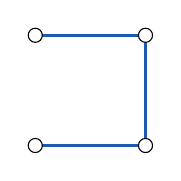
\begin{tikzpicture}[scale=0.7]
\coordinate (p1) at (-1,1);
\coordinate (p2) at (1,-1);
\coordinate (p3) at (1,1);
\coordinate (p4) at (-1,-1);
\draw[edge] (p1) -- (p3);
\draw[edge] (p2) -- (p3);
\draw[edge] (p2) -- (p4);
\node[v] at (p1) {};
\node[v] at (p2) {};
\node[v] at (p3) {};
\node[v] at (p4) {};
\end{tikzpicture}\qquad 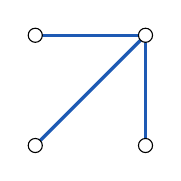
\begin{tikzpicture}[scale=0.7]
\coordinate (p1) at (-1,1);
\coordinate (p2) at (1,-1);
\coordinate (p3) at (1,1);
\coordinate (p4) at (-1,-1);
\draw[edge] (p1) -- (p3);
\draw[edge] (p2) -- (p3);
\draw[edge] (p3) -- (p4);
\node[v] at (p1) {};
\node[v] at (p2) {};
\node[v] at (p3) {};
\node[v] at (p4) {};
\end{tikzpicture}\end{center}\begin{center}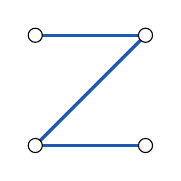
\begin{tikzpicture}[scale=0.7]
\coordinate (p1) at (-1,1);
\coordinate (p2) at (1,-1);
\coordinate (p3) at (1,1);
\coordinate (p4) at (-1,-1);
\draw[edge] (p1) -- (p3);
\draw[edge] (p2) -- (p4);
\draw[edge] (p3) -- (p4);
\node[v] at (p1) {};
\node[v] at (p2) {};
\node[v] at (p3) {};
\node[v] at (p4) {};
\end{tikzpicture}\qquad 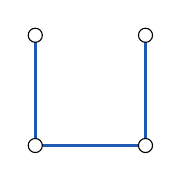
\begin{tikzpicture}[scale=0.7]
\coordinate (p1) at (-1,1);
\coordinate (p2) at (1,-1);
\coordinate (p3) at (1,1);
\coordinate (p4) at (-1,-1);
\draw[edge] (p1) -- (p4);
\draw[edge] (p2) -- (p3);
\draw[edge] (p2) -- (p4);
\node[v] at (p1) {};
\node[v] at (p2) {};
\node[v] at (p3) {};
\node[v] at (p4) {};
\end{tikzpicture}\qquad 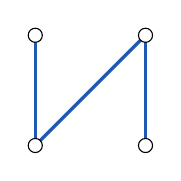
\begin{tikzpicture}[scale=0.7]
\coordinate (p1) at (-1,1);
\coordinate (p2) at (1,-1);
\coordinate (p3) at (1,1);
\coordinate (p4) at (-1,-1);
\draw[edge] (p1) -- (p4);
\draw[edge] (p2) -- (p3);
\draw[edge] (p3) -- (p4);
\node[v] at (p1) {};
\node[v] at (p2) {};
\node[v] at (p3) {};
\node[v] at (p4) {};
\end{tikzpicture}\qquad 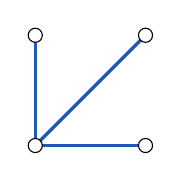
\begin{tikzpicture}[scale=0.7]
\coordinate (p1) at (-1,1);
\coordinate (p2) at (1,-1);
\coordinate (p3) at (1,1);
\coordinate (p4) at (-1,-1);
\draw[edge] (p1) -- (p4);
\draw[edge] (p2) -- (p4);
\draw[edge] (p3) -- (p4);
\node[v] at (p1) {};
\node[v] at (p2) {};
\node[v] at (p3) {};
\node[v] at (p4) {};
\end{tikzpicture}\end{center}\begin{center}Every drawing keeps the same four vertices.\end{center}
\end{frame}

\begin{frame}{Summary: Trees}
\begin{itemize}
  \item \textbf{Structure of trees:} unique paths, leaves, $n-1$ edges, and centers.
  \medskip
  \item \textbf{Spanning trees:} every connected graph contains a spanning tree; Kruskal's algorithm finds one of minimum weight.
  \medskip
  \item \textbf{Counting labeled trees:} Pr\"ufer sequences give a bijective proof of Cayley's formula, $n^{n-2}$.
  \medskip
  \item \textbf{Counting spanning trees:} the Matrix Tree Theorem expresses the answer as any cofactor of $D-A$.
\end{itemize}
\end{frame}

\begin{frame}{Next time: Trails, Circuits, Paths and Cycles}
\begin{center}
\Huge Trails, Circuits,\\[0.4em] Paths and Cycles
\end{center}
\end{frame}

\end{document}
